\section{SoK Methodology}
\label{sec:appendix-methodology}

\subsection{Search Criteria for Literature Review}
\label{sec:keywords}

Web tracking comprises a vast body of literature published over the last few decades---spanning across technical mechanisms, defenses, and regulatory compliance. Through our literature search (see~\autoref{sec:methodology}), we obtained a list of 19438 papers along with their metadata (title, authors, year, and DOI), missing abstracts were completed by performing a DOI-based query on Semantic Scholar\footnote{\url{https://www.semanticscholar.org/}} and OpenAlex\footnote{\url{https://openalex.org/}}.
%
To further filter that list, we first use exclusion keywords to remove potential papers that could be incorrectly retained under web tracking.

\begin{exclusionkeywordbox}
\textbf{Exclusion Keywords:}
\noindent
NOT [\textbf{Title} OR \textbf{abstract}: crypto* OR
blockchain* OR
website fingerprint* OR
``tor'' OR
``poster:'' OR
differential* priva* OR
``federated learning'' OR
``membership inference'' OR
``trusted execution'' OR
``unlearning'' OR
``inversion'' OR
multi-party computation* OR
airtag* OR
privacy label* OR
sdk* OR
``app store'' OR
``google play'' OR
``social media'' OR
smart tv* OR
smart home* OR
``iot'' OR
``virtual reality'' OR
``3g'' OR
``4g'' OR
``5g'' OR
``wireless'' OR
``censorshi''p OR
``voice'' OR
``gaze'' OR
``eye'' OR
``genome'' OR
scam* OR
``bitcoin'' OR
fuzz* OR
cve* OR
certificate authorit* OR
public key* OR
vehicle* OR
robot*]
\end{exclusionkeywordbox}

Second, two sets of inclusion keywords are used to narrow down potential candidates for manual review.
%
The first set is used to filter publications that are related to web tracking techniques and defenses based on their title and abstract text.


\begin{keywordbox}
\textbf{Inclusion Keywords for Techniques and Defenses:}
\noindent
[\textbf{Title} OR \textbf{abstract}: tracking OR
web track* OR
online track* OR
user track* OR
track* user* OR
web privacy OR
online privacy OR
user* privacy OR
user *identifi* OR
track* circumvent* OR
track* eva* OR
track* defen* OR
track* block* OR
ad*block* OR
ad* block*]
\end{keywordbox}


The second set of keywords is used to identify papers discussing privacy regulations and compliance in the context of web tracking in their full text.
%
We rely on full text search to identify papers that may not primarily be regulation-focused (hence lower probability of a match in title or abstract), but may still discuss regulatory implications of the studied tracking technique or defense in the paper.

\begin{keywordbox}
\textbf{Inclusion Keywords for Regulations and Compliance:}
\noindent
[\textbf{Full paper}: regulat* compliance OR
regulation* OR
track* violat* OR
privacy polic* OR
privacy law* OR
privacy regulation* OR
``privacy compliance'' OR
``gdpr'' OR
``ccpa'' OR
``cpra'' OR
``cookie banner'' OR
``cookie compliance'' OR
compliance with cookie* OR
``cookie consent'' OR
track* consent OR
consent management* OR
opt*out OR
opt* out]
\end{keywordbox}

%%
\subsection{Thematic Literature Analysis}
\label{sec:thematic-analysis}
%%


We consider a paper to be a \textit{tracking technique} paper if it provides an in-depth or foundational understanding of a specific tracking mechanism (e.g., first or reference paper on a technique).
%
Similarly, a \textit{tracking defense} paper comprises research that builds a system or an approach to block, prevent, or defend against a tracking technique, while \textit{regulatory compliance} research discusses different aspects of public policies (i.e., privacy regulation, standard, or guideline), their enforcement, and perhaps limitations.
%
Other papers focusing on measuring the prevalence or impact of different tracking techniques are classified as \textit{measurement} research and used throughout this SoK to support systematization of advances in web tracking.
%
This thematic organization is available as part of our artifact (see our~\refopenscience{sec:open-science} statement).

We complement our systematization of research-based tracking defenses with industry-based ones by performing a systematic review of changelogs and release notes for each version of five popular browsers---Brave, Google Chrome, Microsoft Edge (including former Internet Explorer), Mozilla Firefox, and Apple Safari---since their creation.
% ---Brave\footnote{\url{https://github.com/brave/brave-browser/blob/master/CHANGELOG_DESKTOP.md}}, Google Chrome\footnote{\url{https://developer.chrome.com/release-notes}}, Microsoft Edge\footnote{\url{https://learn.microsoft.com/deployedge/microsoft-edge-relnote-archive-stable-channel}} (including former Internet Explorer\footnote{\url{https://learn.microsoft.com/en-us/previous-versions/windows/internet-explorer/ie-developer/dev-guides/}}), Mozilla Firefox\footnote{\url{https://www.mozilla.org/en-US/firefox/releases/}}, and Apple Safari\footnote{\url{https://developer.apple.com/documentation/safari-release-notes} \& \url{https://webkit.org/tracking-prevention/}}---since their creation.
%
Specifically, we extract tracking defense related features across stable versions of browsers based on the description of changes and apply our defense-specific systematization criteria from~\autoref{tab:systematization-criteria} to each defense technique.
%
For each tracking technique and defense technique identified, we also find and associate community-built defenses (if any).

\begin{table*}[ht]
  \small
\centering
\caption{Web tracking artifact taxonomy: mapping of tracked artifacts to artifact labels.}
\label{tab:artifact-taxonomy}
\renewcommand{\arraystretch}{1.2}
\begin{tabular}{@{} p{3.4cm} p{13.8cm} @{}}
\toprule
\textbf{Artifact Label} & \textbf{Artifacts Observed in the Literature Review} \\
\midrule

Browser Storage \& Cache &
  \textit{Cookies};
  \textit{Web Storage} (localStorage, sessionStorage, IndexedDB);
  \textit{Browser Caches} (HTTP, HSTS, favicon, Alt-Svc, Service Worker, and Cache API) \\

\midrule

JavaScript-Accessible Browser APIs &
  \textit{Fingerprinting APIs} (e.g., Navigator, Screen, Canvas, WebGL, AudioContext);
  \textit{Device APIs} (Battery Status, Media Devices, Gamepad, Speech Synthesis voices); 
  \textit{Browser Permissions} (e.g., camera, microphone) \\

\midrule

Hardware Artifacts &
  \textit{GPU Rendering Behavior} (timing variations, memory allocation, performance counters);
  \textit{Sensor Calibration Data} (accelerometer or gyroscope imperfections, speaker frequency response);
  \textit{Clock Drift Patterns} (system time offset, TCP timestamp skew);
  \textit{CPU Microarchitectural State} (scheduling statistics, memory footprint) \\

\midrule

Network Protocol Artifacts &
  \textit{IP Address};
  \textit{TLS/SSL Handshake Parameters} (cipher suites, SNI, client certificates);
  \textit{TCP/IP Stack Characteristics} (source port selection, IP ID fields, IPv6 flow labels);
  \textit{DNS Records} (CNAME records, reverse hostnames, TTL values);
  \textit{QUIC/HTTP2+ Transport Metadata} (connection IDs, retry tokens, transport parameters) \\

\midrule

HTTP Traffic Artifacts &
  Request Metadata, Response Content, Headers, Payload \\

\midrule

Navigational Artifacts &
  \textit{URL Components} (host, domain, path, query parameters);
  \textit{Redirect Chains} \\

\midrule

Webpage Artifacts &
  \textit{Resources} (DOM elements and their modifications, stylesheets, scripts);
  \textit{Interaction Patterns} (click traces, touch gesture characteristics, keystrokes, mouse movements, scroll depth, click coordinates, interaction timing);
  \textit{Rendering Characteristics} (font rendering, CSS feature detection, element bounding dimensions) \\

\midrule

Identifiers &
  \textit{Authentication IDs} (OAuth tokens, SSO redirect parameters, session IDs);
  \textit{PII} (email addresses, phone, PII hashes);
  \textit{Device-specific IDs} (IDFA, EMEI, MAC address); 
  \textit{Advertiser-specific IDs} (e.g., UUIDs)\\

\bottomrule
\end{tabular}
% \vspace{-2mm}
\end{table*}


\newpage
\section{Need for Fingerprinting}
\label{sec:need-for-fingerprinting}

%%
Constructively, fingerprinting can be thought of as a form of intrusion detection.
%
Web applications can learn about the browsing environment or behavior of their first-party users and associate it with specific user identities~\cite{LinPhishSheepsClothing2022}.
%
For example, a website can learn that the user is using a smartphone with specific dimensions or a desktop browser with a specific kind of GPU.
%
If the user's credentials are ever stolen and an attacker attempts to login to that service, the service can extract the attacker's fingerprint, observe a major difference against fingerprints from prior sessions, and request additional authentication data from the attacker (such as a one-time password).
%
The same techniques can be constructively used to differentiate real users from malicious bots or attackers engaging in ad fraud.
%
In practice, large online services commonly incorporate fingerprinting-derived signals into broader abuse-mitigation pipelines to detect automated account creation, credential stuffing, and spam. 
%
These signals are typically combined with behavioral features and rate-limiting mechanisms, enabling services to adapt authentication requirements based on assessed risk and maintaining service integrity in adversarial environments where traditional identifiers are unreliable.

%%
Destructively, the same techniques that can identify user-impersonating attackers and bots, are turned against users who wish to remain anonymous.
%
With fingerprinting, a web app may be able to determine that a certain anonymous user is in fact eponymous, since their browser fingerprint matches that of a known user on the same platform.
%
This undesired re-identification occurs despite user's attempt to hide by deleting cookies or using the browser's private mode.
%
In a cross-site context, fingerprinting can be abused to link unrelated website visits, even when third-party cookies are disabled.


%%
\section{Mixed Tracking}
\label{sec:mixed-tracking}


\subsection{Mixed Tracking Techniques}
\label{sec:mixed-techniques}

%%
Prior stateful and stateless approaches can also be combined to track users across contexts---bridging identity across login boundaries, devices, browsers, and native apps. 
% We refer to these techniques as mixed tracking.

\subsubsection{JavaScript-based Tracking}
\label{sec:mixed-techniques-js-tracking}

%%
% JavaScript is the unifying substrate of both stateful and stateless web tracking. 
%
JavaScript can be used to read and write browser cookies and storage for persistence by stateful techniques while also be used to probe browser APIs to construct a fingerprint by stateless techniques.
%
Although JS-based approaches don't constitute a different tracking technique, it is included here as a canonical example of mixed tracking in practice.


%%
\subsubsection{Authentication-based Tracking}
\label{sec:mixed-techniques-auth-tracking}

%%
Authentication creates a deterministic, cross-context identifier (an account or email address) far more durable than any cookie or fingerprint.
%
Logged-in users are served more third-party trackers and personalized content~\cite{kaizerCharacterizingWebsiteBehaviors2016}, and logged-in pages exhibit more fingerprinting than other pages on the same site, suggesting trackers use authentication to link a stateless fingerprint to stable account identifiers to extend identification into anonymous sessions~\cite{senolDoubleEdgedSword2024}.
%
Moreover, OAuth-based single sign-on itself routinely leaks identifying information to identity providers and relying parties~\cite{dimovaEverybodysLookingSSOmething2023}.
%
As email addresses survive cookie clears and device changes, first parties increasingly hash and share them with advertising partners to build cross-site identity graphs that restore the linkage that third-party cookie restrictions were designed to prevent.


%%
\subsubsection{Cross-device Tracking}
\label{sec:mixed-techniques-cross-device}

%%
When deterministic identifiers are unavailable (e.g., logged out state), trackers fall back to probabilistic signals to link activity across devices---shared IP addresses, browsing patterns~\cite{caoCrossBrowserFingerprintingOS2017}, and behavioral features such as typing dynamics~\cite{yuanCrossdeviceTrackingIdentification2018}.
%
These signals are combined into proprietary \textit{cross-device graphs}, a practice found to be largely opaque to both users and regulators~\cite{zimmeckPrivacyAnalysisCrossdevice2017,brookmanCrossDeviceTrackingMeasurement2017}.
%
Because probabilistic identifiers are inherently noisy (e.g., ISPs dynamically rotate and share public IP addresses across households), trackers apply heuristics such as ignoring commercial, private, and proxied IP ranges or setting temporal thresholds to filter false matches.

%%
\begin{opbox}
Given the lack of ground truth and diversity of proprietary linking algorithms forming cross-device identity graphs, how can cross-device tracking be reliably measured and systematically attributed to uncover specific signals used by different trackers?
\end{opbox}



%%
\subsubsection{Other Cross-Context Tracking}
\label{sec:mixed-techniques-cross-context}

%%
Trackers also bridge contexts within the same device.
%
Cross-browser fingerprinting uses OS- and hardware-level features stable across browsers to link users across browser boundaries~\cite{caoCrossBrowserFingerprintingOS2017}.
%
On mobile, Android Custom Tabs and WebViews share the browser's cookie jar with native apps, letting a tracker plants an identifier in one context that resurfaces in the other, surviving app reinstalls and device backups~\cite{wessels2025hytrack}.
%
% A complementary vector operates without any shared cookie jar, 
Recently, some native apps and in-browser scripts have been found to silently link identities by communicating over \texttt{localhost}, a channel neither the browser's permission model nor the OS sandbox was designed to police~\cite{localmess-usenix-sec-26}.
%
These vectors share a common root cause---OS- and browser-level integration points enabling legitimate app-to-web handoffs that are invisible to in-browser tracking defenses.

%%
\begin{opbox}
Cross-context tracking exploits integration boundaries between browsers, between apps and the web, and between user profiles that no single platform controls end to end. What architectural principles can unify isolation across these boundaries without fragmenting the seamless cross-context experiences users and developers expect?
\end{opbox}





\subsection{Defenses Against Mixed Tracking}
\label{sec:mixed-defenses}


\subsubsection{Industry-based Defenses}
\label{sec:mixed-defenses-industry}


\para{Against Cross-device and Cross-context Tracking.}
%
Deterministic cross-device tracking through shared login accounts is inherently difficult to defend against at the browser level, since the user has explicitly linked their devices by authenticating.
%
Browsers instead address the authentication pathway with purpose-built APIs: the Storage Access API, now shipped by all five major browsers, lets a third party request first-party-equivalent storage explicitly. Chrome and Edge additionally support Federated Credential Management (FedCM), which preserves single sign-on while preventing the identity provider from learning which relying party the user logs into. Brave blocks unrecognized identity providers by default.
%
On mobile, Apple's ATT framework has required explicit opt-in before an app can access the device's advertising identifier since iOS 14.5, and Google's Privacy Sandbox for Android proposed similar restrictions before being abandoned.
%
However, WebViews and in-app browsers share few of the standalone browser's tracking defenses---no extension support, no storage partitioning, no filter-list blocking---leaving users exposed in these embedded contexts.

\begin{opbox}
In cases such as WebViews and in-app browsers, can browser-level tracking protections be extended to embedded rendering engines, or does defense in these contexts require OS-level enforcement that applies regardless of which engine serves the page?
\end{opbox}


%%
\subsubsection{Research-based Defenses}
\label{sec:mixed-defenses-research}



%%
\para{Hardening the Identity Layer.}
%
Because cross-device and authentication-based tracking often runs through a shared identity provider, several proposals harden that layer directly.
%
SPRESSO inserts a forwarder between the relying party and the identity provider so the provider cannot learn which site a user logs into~\cite{fettSPRESSOSecurePrivacyRespecting2015}, encrypted access logging lets a service audit device access without retaining a persistent identifier~\cite{ortegaperezEncryptedAccessLogging2025}, and identity-system reform proposals re-architect national- and platform-level infrastructure to decouple shared identity from cross-service activity correlation~\cite{brandaoMendingTwoNationScale2015}.
% so that the same identity across services does not let those services correlate a user's activity~\cite{brandaoMendingTwoNationScale2015}.


%%
\para{Cryptographic Advertising Proposals.}
%
A parallel line of work shows that measurements advertisers need such as conversion attribution and bid optimization, can be computed without either party learning individual user data.
%
Adnostic, Privad, and ObliviAd demonstrated this for on-device ad selection~\cite{toubianaAdnosticPrivacyPreserving2010,guhaPrivadPracticalPrivacy2011,backesObliviAdProvablySecure2012}, and Ibex later extended the guarantee to conversion attribution and bid optimization jointly using cryptographic aggregation~\cite{zhongIbexPrivacypreservingAd2022}.
%
Few of these designs have been adopted by browser vendors, largely due to computation and coordination costs, but they remain the clearest evidence that interest-based advertising does not inherently require disclosing anything about an individual user.


%%
\subsubsection{Community-based Defenses}
\label{sec:mixed-defenses-community}


\para{Universal Opt-out Signals.}
%
Several attempts were made at implementing opt out and consent signals for users to communicate their privacy preferences to services. However, the adoption and enforcement of such signals by both senders and recipients is an unresolved coordination problem~\cite{hilsPrivacyPreferenceSignals2021}.

%%
\noindent
\textit{Platform for Privacy Preferences Project (P3P)}~\cite{reaglePlatformPrivacyPreferences1999,cranorPlatformPrivacyPreferences2002,byersSearchingPrivacyDesign2005,cranorPlatformPrivacyPreferences2006} enabled websites to communicate their privacy practices to users in a standardized and fine-grained format.
%
The P3P specification was published by the W3C in 2002, but was rapidly criticized for being too complex to implement or understand.
%
Its utility was limited by the low number of sites that were adopting it~\cite{cranorUseP3PUser2002} and those implementing it correctly and transparently~\cite{cranorAnalysisP3PDeployment2003, leonTokenAttemptMisrepresentation2010}.
%
Ultimately, the specification was officially obsoleted by the W3C in 2018.

\noindent
\textit{Do Not Track (DNT)}~\cite{fieldingTrackingPreferenceExpression2019}, proposed in 2009 as a binary opt out signal, was adopted by every major browser but was never given legal force.
%
Indeed, CalOPPA, which influenced the design of DNT, only requires online services to say whether or not they respect it~\cite{CaliforniaCodeBPC2003}.
%
The W3C working group for DNT closed in 2019 without industry consensus.

\noindent\textit{Global Privacy Control (GPC)}~\cite{zimmeckGlobalPrivacyControl2024} can be viewed as a successor to DNT, but succeeds where DNT failed by being legally enforceable: California's 2022 settlement with Sephora~\cite{bontaAttorneyGeneralBonta2022} established that ignoring GPC violates the CCPA~\cite{attorneygeneralbecerraCCPARequiresBusinesses2021}, and Colorado has since imposed a similar requirement in 2024~\cite{coloradodepartmentoflawUniversalOptOutShortlist2024}.
%
Additional recognition of universal opt outs by states like Connecticut, Montana, Oregon, and Texas is driving broader adoption than DNT ever achieved, although it is still slow despite people finding the signal useful and usable~\cite{zimmeckUsabilityEnforceabilityGlobal2023,zimmeckGeneralizableActivePrivacy2024,azizJohnnyStillCant2024}.
%
DuckDuckGo, Brave, and Firefox send GPC by default; Chrome added support only in 2026~\cite{googleGlobalPrivacyControl2025}.
%
As GPC is not tied to any single storage or fingerprinting mechanism, it acts as a cross-cutting signal that covers every technique discussed in this SoK, given a site honors it.

\begin{opbox}
The applicability of GPC in the EU within ePD and GDPR context is an open discussion~\cite{berjonGPCGDPR2021,bielovaEffectDesignPatterns2024
}. Will EU regulators incorporate GPC as an opt-out signal? 
\end{opbox}



% \newpage
\newlength{\artfirstcol}
\newlength{\artdatacol}

\setlength{\artfirstcol}{2.6cm} % <- change to widen/narrow first column
\setlength{\artdatacol}{0.58cm}  % <- widen data columns so Navigation fits in 2-col span

\newcolumntype{T}{>{\centering\arraybackslash}b{\artdatacol}}
\newcolumntype{Z}{>{\centering\arraybackslash}b{\artdatacol}}


\newcommand{\gtick}{\textcolor{green!50!black}{\checkmark}}

\begin{table*}[ht] %[!t]
\centering
\scriptsize
\setlength{\tabcolsep}{0.6pt}
\resizebox{\textwidth}{!}{%
\begin{tabular}{%
>{\raggedright\arraybackslash}m{\artfirstcol}|%
>{\centering\arraybackslash}m{1.4cm}|%    Venue Year
*{24}{T}%
}
 
\toprule
\multicolumn{1}{>{\centering\arraybackslash}b{\artfirstcol}|}{\shortstack[c]{\textbf{Tracking Technique}\\\textbf{Literature}}} & \multicolumn{1}{>{\centering\arraybackslash}b{1.4cm}|}{\shortstack[c]{\textbf{Venue}\\\textbf{Year}}} & \multicolumn{1}{Z}{\rot{Third-party Cookie Tracking}} & \multicolumn{1}{Z}{\rot{Cookie Respawning}} & \multicolumn{1}{Z}{\rot{Cookie Syncing}} & \multicolumn{1}{Z}{\rot{First-party Cookie Tracking}} & \multicolumn{1}{Z}{\rot{Tracking Pixels/Tags}} & \multicolumn{1}{Z}{\rot{CNAME Tracking}} & \multicolumn{1}{Z}{\rot{Server-side Tracking}} & \multicolumn{1}{Z}{\rot{Link Decorations}} & \multicolumn{1}{Z}{\rot{Bounce Tracking}} & \multicolumn{1}{Z}{\rot{Authentication-based Tracking}} & \multicolumn{1}{Z}{\rot{Javascript-based Tracking}} & \multicolumn{1}{Z}{\rot{Browser Fingerprinting}} & \multicolumn{1}{Z}{\rot{Browser Extension Fingerprinting}} & \multicolumn{1}{Z}{\rot{Device Fingerprinting}} & \multicolumn{1}{Z}{\rot{Passive Fingerprinting}} & \multicolumn{1}{Z}{\rot{Kernel-based Side-channels}} & \multicolumn{1}{Z}{\rot{Network-based Side-channels}} & \multicolumn{1}{Z}{\rot{Storage-based Side-channels}} & \multicolumn{1}{Z}{\rot{Timing-based Side-channels}} & \multicolumn{1}{Z}{\rot{Behavioral Tracking}} & \multicolumn{1}{Z}{\rot{Cross-context Tracking}} & \multicolumn{1}{Z}{\rot{FLoC / Topics API}} & \multicolumn{1}{Z}{\rot{Protected Audience}} & \multicolumn{1}{Z}{\rot{Ad-Blocking Circumvention}} \\
\midrule
Felten et al.~\cite{feltenTimingAttacksWeb2000} &  CCS'00 &   &   &   &   &   &   &   &   &   &   &   &   &   &   &   &   &   &   &  \scalebox{1.15}{\textbf{\gtick}} &   &   &   &   &   \\
Kohno et al.~\cite{kohnoRemotePhysicalDevice2005} &  S\&P'05 &   &   &   &   &   &   &   &   &   &   &   &   &   &  \scalebox{1.15}{\textbf{\gtick}} &   &   &   &   &   &   &   &   &   &   \\
Chen et al.~\cite{chenSideChannelLeaksWeb2010} &  S\&P'10 &   &   &   &   &   &   &   &   &   &   &   &   &   &   &   &   &  \scalebox{1.15}{\textbf{\gtick}} &   &   &   &   &   &   &   \\
Yen et al.~\cite{yenHostFingerprintingTracking2012} &  NDSS'12 &   &   &   &   &   &   &   &   &   &   &   &  \scalebox{1.15}{\textbf{\gtick}} &   &  \scalebox{1.15}{\textbf{\gtick}} &   &   &   &   &   &   &   &   &   &   \\
Jana et al.~\cite{janaMementoLearningSecrets2012} &  S\&P'12 &   &   &   &   &   &   &   &   &   &   &   &   &   &   &   &  \scalebox{1.15}{\textbf{\gtick}} &   &   &   &   &   &   &   &   \\
Nikiforakis et al.~\cite{nikiforakisCookielessMonsterExploring2013} &  S\&P'13 &   &   &   &   &   &   &  \scalebox{1.15}{\textbf{\gtick}} &   &   &   &   &   &   &  \scalebox{1.15}{\textbf{\gtick}} &   &   &   &   &   &   &   &   &   &   \\
Acar et al.~\cite{acarWebNeverForgets2014} &  CCS'14 &   &  \scalebox{1.15}{\textbf{\gtick}} &  \scalebox{1.15}{\textbf{\gtick}} &   &   &   &   &   &   &   &  \scalebox{1.15}{\textbf{\gtick}} &  \scalebox{1.15}{\textbf{\gtick}} &   &   &   &   &   &   &   &   &   &   &   &   \\
Zhou et al.~\cite{zhouAcousticFingerprintingRevisited2014} &  CCS'14 &   &   &   &   &   &   &   &   &   &   &   &   &   &  \scalebox{1.15}{\textbf{\gtick}} &   &   &   &   &   &   &   &   &   &   \\
Oren et al.~\cite{orenSpySandboxPractical2015} &  CCS'15 &   &   &   &   &   &   &   &   &   &   &   &   &   &   &   &   &   &   &  \scalebox{1.15}{\textbf{\gtick}} &   &   &   &   &   \\
Das et al.~\cite{dasWebsSixthSense2018, dasTrackingMobileWeb2016, dasEveryMoveYou2018} &  NDSS'16 &   &   &   &   &   &   &   &   &   &   &  \scalebox{1.15}{\textbf{\gtick}} &   &   &  \scalebox{1.15}{\textbf{\gtick}} &   &   &   &   &   &   &   &   &   &   \\
Laperdrix et al.~\cite{laperdrixBeautyBeastDiverting2016} &  S\&P'16 &   &   &   &   &   &   &  \scalebox{1.15}{\textbf{\gtick}} &   &   &   &   &  \scalebox{1.15}{\textbf{\gtick}} &   &   &   &   &   &   &   &   &   &   &   &   \\
Jain et al.~\cite{jainMiningLatentClient2016} &  PETS'16 &   &   &   &   &   &   &   &   &   &   &   &   &   &   &   &   &  \scalebox{1.15}{\textbf{\gtick}} &   &   &   &   &   &   &   \\
Gonzalez et al.~\cite{gonzalezUserProfilingTime2016} &  IMC'16 &   &   &   &   &   &   &   &   &   &   &   &   &   &   &   &   &  \scalebox{1.15}{\textbf{\gtick}} &   &   &   &   &   &   &   \\
Kaizer et al.~\cite{kaizerCharacterizingWebsiteBehaviors2016} &  IMC'16 &   &   &   &  \scalebox{1.15}{\textbf{\gtick}} &   &   &   &   &   &  \scalebox{1.15}{\textbf{\gtick}} &  \scalebox{1.15}{\textbf{\gtick}} &   &   &   &   &   &   &   &   &  \scalebox{1.15}{\textbf{\gtick}} &   &   &   &   \\
Cao et al.~\cite{caoCrossBrowserFingerprintingOS2017} &  NDSS'17 &   &   &   &   &   &   &   &   &   &   &  \scalebox{1.15}{\textbf{\gtick}} &   &   &  \scalebox{1.15}{\textbf{\gtick}} &   &   &   &   &   &   &   &   &   &   \\
Starov et al.~\cite{starovXHOUNDQuantifyingFingerprintability2017} &  S\&P'17 &   &   &   &   &   &   &  \scalebox{1.15}{\textbf{\gtick}} &   &   &   &   &   &  \scalebox{1.15}{\textbf{\gtick}} &   &   &   &   &   &   &   &   &   &   &   \\
Vastel et al.~\cite{vastelFPSTALKERTrackingBrowser2018} &  S\&P'18 &   &   &   &   &   &   &  \scalebox{1.15}{\textbf{\gtick}} &   &   &   &   &  \scalebox{1.15}{\textbf{\gtick}} &   &   &   &   &   &   &   &   &   &   &   &   \\
Foppe et al.~\cite{foppeExploitingTLSClient2018} &  PETS'18 &   &   &   &   &   &   &   &   &   &   &   &   &   &   &   &   &  \scalebox{1.15}{\textbf{\gtick}} &   &   &   &   &   &   &   \\
Masood et al.~\cite{masoodTouchYoureTrappcked2018} &  PETS'18 &   &   &   &   &   &   &   &   &   &   &  \scalebox{1.15}{\textbf{\gtick}} &   &   &   &   &   &   &   &   &  \scalebox{1.15}{\textbf{\gtick}} &   &   &   &   \\
Olejnik et al.~\cite{olejnikLeakingBatteryPrivacy2016} &  USENIX'18 &   &   &   &   &   &   &   &   &   &   &  \scalebox{1.15}{\textbf{\gtick}} &  \scalebox{1.15}{\textbf{\gtick}} &   &   &   &   &   &   &   &   &   &   &   &   \\
Bashir et al.~\cite{bashirHowTrackingCompanies2018} &  IMC'18 &   &   &   &   &   &   &   &   &   &   &  \scalebox{1.15}{\textbf{\gtick}} &   &   &   &   &   &   &   &   &   &   &   &   &  \scalebox{1.15}{\textbf{\gtick}} \\
Klein et al.~\cite{klein2019dns} &  NDSS'19 &   &   &   &   &   &   &   &   &   &   &  \scalebox{1.15}{\textbf{\gtick}} &   &   &   &   &   &   &  \scalebox{1.15}{\textbf{\gtick}} &   &   &   &   &   &   \\
Hu et al.~\cite{huCharacterizingPixelTracking2019} &  S\&P'19 &   &   &   &   &   &  \scalebox{1.15}{\textbf{\gtick}} &   &   &   &   &   &   &   &   &   &   &   &   &   &   &   &   &   &   \\
Martin et al.~\cite{martinHandoffAllYour2019} &  PETS'19 &   &   &   &   &   &   &   &   &   &   &   &   &   &  \scalebox{1.15}{\textbf{\gtick}} &   &   &   &   &   &   &   &   &   &   \\
Sy et al.~\cite{syQUICLookWeb2019} &  PETS'19 &   &   &   &   &   &   &   &   &   &   &   &   &   &   &   &   &  \scalebox{1.15}{\textbf{\gtick}} &  \scalebox{1.15}{\textbf{\gtick}} &   &   &   &   &   &   \\
Karami et al.~\cite{karamiCarnusExploringPrivacy2020} &  NDSS'20 &   &   &   &   &   &   &   &   &   &   &  \scalebox{1.15}{\textbf{\gtick}} &   &  \scalebox{1.15}{\textbf{\gtick}} &   &   &   &   &   &   &   &   &   &   &   \\
Koop et al.~\cite{koopInDepthEvaluationRedirect2020} &  PETS'20 &   &   &   &   &   &   &   &  \scalebox{1.15}{\textbf{\gtick}} &   &   &   &   &   &   &   &   &   &   &   &   &   &   &   &   \\
Li et al.~\cite{liShimShimmenyEvaluating2020} &  USENIX'20 &   &   &   &   &   &   &   &  \scalebox{1.15}{\textbf{\gtick}} &   &   &   &   &   &   &   &   &   &   &   &   &   &   &   &   \\
Mishra et al.~\cite{mishraDontCountMe2020} &  WWW'20 &   &   &   &   &   &   &   &   &   &   &   &   &   &   &  \scalebox{1.15}{\textbf{\gtick}} &   &   &   &   &   &   &   &   &   \\
Solomos et al.~\cite{solomosTalesFaviconsCaches2021} &  NDSS'21 &   &   &   &   &   &   &   &   &   &   &   &   &   &   &   &   &   &  \scalebox{1.15}{\textbf{\gtick}} &   &   &   &   &   &   \\
Klein et al.~\cite{kleinCrossLayerAttacks2021} &  S\&P'21 &   &   &   &   &   &   &   &   &   &   &   &   &   &  \scalebox{1.15}{\textbf{\gtick}} &   &  \scalebox{1.15}{\textbf{\gtick}} &   &   &   &   &   &   &   &   \\
Dimova et al.~\cite{dimovaCNAMEGameLargescale2021} &  PETS'21 &   &   &   &   &   &  \scalebox{1.15}{\textbf{\gtick}} &   &   &   &   &  \scalebox{1.15}{\textbf{\gtick}} &   &   &   &   &   &   &   &   &   &   &   &   &   \\
Mishra et al.~\cite{mishraDejaVuAbusing2021} &  PETS'21 &   &   &   &   &   &   &   &   &   &   &   &   &   &   &   &   &   &  \scalebox{1.15}{\textbf{\gtick}} &   &   &   &   &   &   \\
Laperdrix et al.~\cite{laperdrixFingerprintingStyleDetecting2021} &  USENIX'21 &   &   &   &   &   &   &   &   &   &   &  \scalebox{1.15}{\textbf{\gtick}} &   &  \scalebox{1.15}{\textbf{\gtick}} &   &   &   &   &   &   &   &   &   &   &   \\
Chen et al.~\cite{chenCookieSwapParty2021} &  WWW'21 &   &   &   &  \scalebox{1.15}{\textbf{\gtick}} &   &   &   &   &   &   &  \scalebox{1.15}{\textbf{\gtick}} &   &   &   &   &   &   &   &   &   &   &   &   &   \\
Rye et al.~\cite{ryeFollowScentDefeating2021} &  IMC'21 &   &   &   &   &   &   &   &   &   &   &   &   &   &   &  \scalebox{1.15}{\textbf{\gtick}} &   &   &   &   &   &   &   &   &   \\
Laor et al.~\cite{laorDRAWNAPARTDevice2022} &  NDSS'22 &   &   &   &   &   &   &   &   &   &   &  \scalebox{1.15}{\textbf{\gtick}} &   &   &  \scalebox{1.15}{\textbf{\gtick}} &   &   &   &   &   &   &   &   &   &   \\
Jin et al.~\cite{jinTimingBasedBrowsingPrivacy2022} &  S\&P'22 &   &   &   &   &   &   &  \scalebox{1.15}{\textbf{\gtick}} &   &   &   &   &   &   &   &   &   &   &   &  \scalebox{1.15}{\textbf{\gtick}} &   &   &   &   &   \\
Khodayari et al.~\cite{khodayariStateSameSiteStudying2022} &  S\&P'22 &  \scalebox{1.15}{\textbf{\gtick}} &   &   &  \scalebox{1.15}{\textbf{\gtick}} &   &   &   &   &   &   &   &   &   &   &   &   &   &   &   &   &   &   &   &   \\
Randall et al.~\cite{randallMeasuringUIDSmuggling2022} &  IMC'22 &   &   &   &   &   &   &   &   &  \scalebox{1.15}{\textbf{\gtick}} &   &  \scalebox{1.15}{\textbf{\gtick}} &   &   &   &   &   &   &   &   &   &   &   &   &   \\
Berke et al.~\cite{berkePrivacyLimitationsInterestbased2022} &  CCS'22 &   &   &   &   &   &   &   &   &   &   &  \scalebox{1.15}{\textbf{\gtick}} &   &   &   &   &   &   &   &   &   &   &  \scalebox{1.15}{\textbf{\gtick}} &   &   \\
Solomos et al.~\cite{solomosEscapingConfinesTime2022} &  CCS'22 &   &   &   &   &   &   &   &   &   &   &  \scalebox{1.15}{\textbf{\gtick}} &   &  \scalebox{1.15}{\textbf{\gtick}} &   &   &   &   &   &   &   &   &   &   &   \\
Ali et al.~\cite{aliNavigatingMurkyWaters2023} &  NDSS'23 &   &   &   &   &   &   &   &   &   &   &  \scalebox{1.15}{\textbf{\gtick}} &   &   &   &   &   &   &  \scalebox{1.15}{\textbf{\gtick}} &   &   &   &   &  \scalebox{1.15}{\textbf{\gtick}} &   \\
Nomoto et al.~\cite{nomoto2023browser} &  NDSS'23 &   &   &   &   &   &   &   &   &   &   &  \scalebox{1.15}{\textbf{\gtick}} &  \scalebox{1.15}{\textbf{\gtick}} &   &   &   &   &   &   &   &   &   &   &   &   \\
Lin et al.~\cite{linFashionFauxPas2023} &  S\&P'23 &   &   &   &   &   &   &  \scalebox{1.15}{\textbf{\gtick}} &   &   &   &   &  \scalebox{1.15}{\textbf{\gtick}} &   &   &   &   &   &   &   &   &   &   &   &   \\
Jha et al.~\cite{jhaRobustnessTopicsAPI2023} &  PETS'23 &   &   &   &   &   &   &   &   &   &   &  \scalebox{1.15}{\textbf{\gtick}} &   &   &   &   &   &   &   &   &   &   &  \scalebox{1.15}{\textbf{\gtick}} &   &   \\
Kol et al.~\cite{kol2023device} &  USENIX'23 &   &   &   &   &   &   &   &   &   &   &   &   &   &  \scalebox{1.15}{\textbf{\gtick}} &   &  \scalebox{1.15}{\textbf{\gtick}} &   &   &   &   &   &   &   &   \\
Snyder et al.~\cite{snyderPoolPartyExploitingBrowser2023} &  USENIX'23 &   &   &   &   &   &   &   &   &   &   &  \scalebox{1.15}{\textbf{\gtick}} &   &   &   &   &   &   &  \scalebox{1.15}{\textbf{\gtick}} &   &   &  \scalebox{1.15}{\textbf{\gtick}} &   &   &   \\
Su et al.~\cite{suAutomaticDiscoveryEmerging2023} &  WWW'23 &   &   &   &   &   &   &   &   &   &   &  \scalebox{1.15}{\textbf{\gtick}} &  \scalebox{1.15}{\textbf{\gtick}} &   &   &   &   &   &   &   &   &   &   &   &   \\
Beugin et al.~\cite{beuginInterestdisclosingMechanismsAdvertising2024} &  PETS'24 &   &   &   &   &   &   &   &   &   &   &  \scalebox{1.15}{\textbf{\gtick}} &   &   &   &   &   &   &   &   &   &   &  \scalebox{1.15}{\textbf{\gtick}} &   &   \\
Fouad et al.~\cite{fouadDevilDetailsDetection2024} &  PETS'24 &   &   &   &   &   &   &  \scalebox{1.15}{\textbf{\gtick}} &   &   &   &   &   &   &   &   &   &   &   &   &   &   &   &   &   \\
Chehade et al.~\cite{chehade2025double} &  USENIX'25 &   &   &   &   &   &   &   &   &   &   &  \scalebox{1.15}{\textbf{\gtick}} &   &  \scalebox{1.15}{\textbf{\gtick}} &   &   &   &   &   &   &   &   &   &   &   \\
Wessels et al.~\cite{wessels2025hytrack} &  USENIX'25 &   &  \scalebox{1.15}{\textbf{\gtick}} &   &   &   &   &   &   &   &   &   &   &   &   &   &   &   &   &   &   &  \scalebox{1.15}{\textbf{\gtick}} &   &   &   \\
Huyghe et al.~\cite{huygheFPRainbowFingerprintBasedBrowser2025} &  WWW'25 &   &   &   &   &   &   &   &   &   &   &  \scalebox{1.15}{\textbf{\gtick}} &  \scalebox{1.15}{\textbf{\gtick}} &   &   &   &   &   &   &   &   &   &   &   &   \\
Bekos et al.~\cite{bekosPIIxelLeaksPassive2025} &  CCS'25 &   &   &   &   &  \scalebox{1.15}{\textbf{\gtick}} &   &   &   &   &   &  \scalebox{1.15}{\textbf{\gtick}} &   &   &   &   &   &   &   &   &   &   &   &   &   \\
Ukani et al.~\cite{ukaniLocalFramesExploiting2025} &  CCS'25 &  \scalebox{1.15}{\textbf{\gtick}} &   &   &   &   &   &   &   &   &   &  \scalebox{1.15}{\textbf{\gtick}} &  \scalebox{1.15}{\textbf{\gtick}} &   &   &   &   &   &   &   &   &   &   &   &  \scalebox{1.15}{\textbf{\gtick}} \\
 
\bottomrule
\end{tabular}%
}% end resizebox
\caption{Literature on papers studying web tracking techniques over the years.}
\label{tab:technique-papers}
\end{table*}


% \newpage
\begin{table}[!t]
\centering
\scriptsize
\setlength{\tabcolsep}{0.6pt}
\renewcommand{\arraystretch}{1.0}
\begin{tabular}{%
>{\raggedright\arraybackslash}m{2.6cm}|%
*{8}{>{\centering\arraybackslash}m{0.7cm}}%
}

\toprule
\multicolumn{1}{>{\centering\arraybackslash}b{2.6cm}|}{\shortstack[c]{\textbf{Tracking Technique}\\\textbf{Literature}}} & \multicolumn{1}{>{\centering\arraybackslash}b{0.7cm}}{\rot{Browser Storage and Cache}} & \multicolumn{1}{>{\centering\arraybackslash}b{0.7cm}}{\rot{JavaScript-Accessible Browser APIs}} & \multicolumn{1}{>{\centering\arraybackslash}b{0.7cm}}{\rot{Webpage Artifacts}} & \multicolumn{1}{>{\centering\arraybackslash}b{0.7cm}}{\rot{Hardware Artifacts}} & \multicolumn{1}{>{\centering\arraybackslash}b{0.7cm}}{\rot{Network Protocol Artifacts}} & \multicolumn{1}{>{\centering\arraybackslash}b{0.7cm}}{\rot{HTTP Traffic Artifacts}} & \multicolumn{1}{>{\centering\arraybackslash}b{0.7cm}}{\rot{Navigational Artifacts}} & \multicolumn{1}{>{\centering\arraybackslash}b{0.7cm}}{\rot{Identifiers}} \\
\midrule
Felten et al.~\cite{feltenTimingAttacksWeb2000} & {\symStorage} & {\symExecution} & {\symInclusion} &  &  &  &  & \\
Kohno et al.~\cite{kohnoRemotePhysicalDevice2005} &  &  &  & {\symObservation} & {\symObservation} &  &  & \\
Chen et al.~\cite{chenSideChannelLeaksWeb2010} &  &  &  &  & {\symObservation} &  &  & \\
Yen et al.~\cite{yenHostFingerprintingTracking2012} & {\symStorage} & {\symExecution} & {\symInclusion} &  & {\symObservation} & {\symInclusion\,\symSharing} &  & {\symObservation} \\
Jana et al.~\cite{janaMementoLearningSecrets2012} &  &  &  & {\symObservation} & &  &  & \\
Nikiforakis et al.~\cite{nikiforakisCookielessMonsterExploring2013} &  & {\symExecution} & {\symInclusion\,\symExecution} &  &  & {\symInclusion\,\symSharing} &  & \\
Zhou et al.~\cite{zhouAcousticFingerprintingRevisited2014} &  &  &  & {\symExecution} &  &  &  & \\
Acar et al.~\cite{acarWebNeverForgets2014} & {\symStorage} & {\symExecution} & {\symInclusion\,\symExecution} &  &  & {\symInclusion\,\symSharing} & {\symSharing} & {\symStorage\,\symSharing}\\
Oren et al.~\cite{orenSpySandboxPractical2015} &  & {\symExecution} &  & {\symExecution} &  &  &  & \\
Das et al.~\cite{dasWebsSixthSense2018, dasTrackingMobileWeb2016, dasEveryMoveYou2018} &  & {\symExecution} &  & {\symExecution} &  &  &  & \\
Laperdrix et al.~\cite{laperdrixBeautyBeastDiverting2016} &  & {\symExecution} & {\symInclusion\,\symExecution} &  &  & {\symInclusion\,\symSharing} &  & \\
Jain et al.~\cite{jainMiningLatentClient2016} &  &  &  &  & {\symObservation} &  &  & {\symObservation}\\
Gonzalez et al.~\cite{gonzalezUserProfilingTime2016} &  &  &  &  & {\symObservation} & {\symObservation} &  & \\
Kaizer et al.~\cite{kaizerCharacterizingWebsiteBehaviors2016} & {\symStorage} &  & {\symInclusion\,\symExecution} &  &  & {\symInclusion\,\symSharing} &  & {\symStorage}\\
Cao et al.~\cite{caoCrossBrowserFingerprintingOS2017} &  & {\symExecution} & {\symInclusion\,\symExecution} & {\symExecution} &  &  &  & \\
Starov et al.~\cite{starovXHOUNDQuantifyingFingerprintability2017} &  &  & {\symInclusion\,\symExecution} &  &  &  &  & \\
Vastel et al.~\cite{vastelFPSTALKERTrackingBrowser2018} &  & {\symExecution} & {\symInclusion\,\symExecution} &  &  & {\symInclusion\,\symSharing} &  & \\
Foppe et al.~\cite{foppeExploitingTLSClient2018} &  &  &  &  & {\symObservation} &  &  & {\symObservation}\\
Masood et al.~\cite{masoodTouchYoureTrappcked2018} &  & {\symExecution} & {\symInclusion\,\symExecution} &  &  &  &  & \\
Olejnik et al.~\cite{olejnikLeakingBatteryPrivacy2016} &  & {\symExecution} &  &  &  &  &  & \\
Bashir et al.~\cite{bashirHowTrackingCompanies2018} & {\symStorage} & {\symExecution} & {\symInclusion} &  &  & {\symInclusion\,\symSharing} &  & \\
Klein et al.~\cite{klein2019dns} &  & {\symExecution} & {\symInclusion} &  & {\symObservation} &  &  & \\
Hu et al.~\cite{huCharacterizingPixelTracking2019} & {\symStorage} &  & {\symInclusion} &  &  & {\symInclusion\,\symSharing} & {\symSharing} & {\symStorage\,\symSharing}\\
Sy et al.~\cite{syQUICLookWeb2019} &  &  &  &  & {\symObservation} &  &  & {\symObservation}\\
Martin et al.~\cite{martinHandoffAllYour2019} &  & &  & {\symObservation} &  &  &  & {\symObservation}\\
Karami et al.~\cite{karamiCarnusExploringPrivacy2020} &  &  & {\symInclusion\,\symExecution} &  &  & {\symInclusion\,\symSharing} &  & \\
Koop et al.~\cite{koopInDepthEvaluationRedirect2020} & {\symStorage} &  & {\symInclusion} &  &  &  & {\symSharing} & \\
Li et al.~\cite{liShimShimmenyEvaluating2020} &  &  & {\symInclusion} &  &  & {\symInclusion\,\symSharing} & {\symSharing} & \\
Mishra et al.~\cite{mishraDontCountMe2020} & {\symStorage} &  &  &  & {\symObservation} & {\symInclusion\,\symSharing} &  & \\
Solomos et al.~\cite{solomosTalesFaviconsCaches2021} & {\symStorage} &  &  &  &  &  &  & \\
Klein et al.~\cite{kleinCrossLayerAttacks2021} &  &  &  & {\symObservation} & {\symObservation} &  &  & \\
Mishra et al.~\cite{mishraDejaVuAbusing2021} & {\symStorage} &  & {\symInclusion} &  &  & {\symInclusion\,\symSharing} &  & \\
Dimova et al.~\cite{dimovaCNAMEGameLargescale2021} & {\symStorage} &  & {\symInclusion} &  & {\symSharing} & {\symInclusion\,\symSharing} &  & \\
Laperdrix et al.~\cite{laperdrixFingerprintingStyleDetecting2021} &  & {\symExecution} & {\symInclusion\,\symExecution} &  &  &  &  & \\
Chen et al.~\cite{chenCookieSwapParty2021} & {\symStorage} &  & {\symInclusion\,\symExecution} &  &  & {\symInclusion\,\symSharing} &  & \\
Rye et al.~\cite{ryeFollowScentDefeating2021} &  &  &  &  & {\symObservation} &  &  & \\
Laor et al.~\cite{laorDRAWNAPARTDevice2022} &  & {\symExecution} & {\symInclusion\,\symExecution} & {\symExecution} &  &  &  & \\
Khodayari et al.~\cite{khodayariStateSameSiteStudying2022} & {\symStorage} &  &  &  &  & {\symSharing} &  & \\
Jin et al.~\cite{jinTimingBasedBrowsingPrivacy2022} &  & {\symExecution} &  & {\symExecution} &  &  &  & \\
Randall et al.~\cite{randallMeasuringUIDSmuggling2022} & {\symStorage} & {\symExecution} & {\symInclusion\,\symExecution} &  &  & {\symInclusion\,\symSharing} & {\symSharing} & {\symStorage\,\symSharing}\\
Berke et al.~\cite{berkePrivacyLimitationsInterestbased2022} &  & {\symExecution} &  &  &  &  &  & \\
Solomos et al.~\cite{solomosEscapingConfinesTime2022} &  & {\symExecution} & {\symInclusion\,\symExecution} &  &  &  &  & \\
Nomoto et al.~\cite{nomoto2023browser} &  & {\symExecution} &  &  &  &  &  & \\
Ali et al.~\cite{aliNavigatingMurkyWaters2023} & {\symStorage} &  &  &  &  &  &  & \\
Lin et al.~\cite{linFashionFauxPas2023} &  & {\symExecution} & {\symInclusion\,\symExecution} &  &  &  &  & \\
Jha et al.~\cite{jhaRobustnessTopicsAPI2023} &  & {\symExecution} &  &  &  &  &  & \\
Kol et al.~\cite{kol2023device} &  &  &  & {\symObservation} & {\symObservation} &  &  & \\
Snyder et al.~\cite{snyderPoolPartyExploitingBrowser2023} & {\symStorage} & {\symExecution} &  &  &  &  &  & \\
Su et al.~\cite{suAutomaticDiscoveryEmerging2023} &  & {\symExecution} & {\symInclusion\,\symExecution} &  &  &  &  & \\
Beugin et al.~\cite{beuginInterestdisclosingMechanismsAdvertising2024} &  & {\symExecution} &  &  &  &  &  & \\
Fouad et al.~\cite{fouadDevilDetailsDetection2024} & {\symStorage} &  & {\symInclusion} &  & {\symSharing} & {\symInclusion\,\symSharing} &  & \\
Chehade et al.~\cite{chehade2025double} &  &  & {\symInclusion\,\symExecution} &  &  & {\symInclusion\,\symSharing} &  & \\
Wessels et al.~\cite{wessels2025hytrack} & {\symStorage} &  &  &  &  &  &  & {\symStorage}\\
Huyghe et al.~\cite{huygheFPRainbowFingerprintBasedBrowser2025} &  & {\symExecution} & {\symInclusion\,\symExecution} &  &  &  &  & \\
Ukani et al.~\cite{ukaniLocalFramesExploiting2025} & {\symStorage} & {\symExecution} & {\symInclusion\,\symExecution} &  &  &  &  & \\
Bekos et al.~\cite{bekosPIIxelLeaksPassive2025} & {\symStorage} & {\symExecution} & {\symInclusion\,\symExecution} &  &  & {\symInclusion\,\symSharing} & {\symSharing} & \\

\bottomrule
\end{tabular}
\caption{Tracker capabilities exercised over artifacts as studied in each tracking techniques related paper.}
\label{tab:paper-artifacts}
\end{table}
\newcommand{\cmark}{\scalebox{1.15}{\textbf{\gtick}}}

\begin{table}[!t]
\centering
\scriptsize
\setlength{\tabcolsep}{0.5pt}
\renewcommand{\arraystretch}{0.94}
\begin{tabular}{%
>{\raggedright\arraybackslash}m{3.4cm}|%
>{\centering\arraybackslash}m{1.5cm}|%
>{\centering\arraybackslash}m{0.7cm}|%
*{8}{>{\centering\arraybackslash}m{0.3cm}}%
}

\toprule
\multicolumn{1}{>{\centering\arraybackslash}b{3.4cm}|}{\shortstack[c]{\textbf{Tracking Defense}\\\textbf{Literature}\\\textbf{(Defense System Name)}}} &
\multicolumn{1}{>{\centering\arraybackslash}b{1.5cm}|}{\shortstack[c]{\textbf{Venue}\\\textbf{Year}}} &
\multicolumn{1}{>{\centering\arraybackslash}b{0.7cm}|}{\rot{Deployment Type}} &
\multicolumn{1}{>{\cellcolor{cellred}\centering\arraybackslash}b{0.32cm}}{\rot{ML-based}} &
\multicolumn{1}{>{\cellcolor{cellred}\centering\arraybackslash}b{0.32cm}}{\rot{Program Instrum.}} &
\multicolumn{1}{>{\cellcolor{cellred}\centering\arraybackslash}b{0.32cm}}{\rot{Circumvention-based}} &
\multicolumn{1}{>{\cellcolor{cellred}\centering\arraybackslash}b{0.32cm}}{\rot{LLM-based}} &
\multicolumn{1}{>{\cellcolor{cellyellow}\centering\arraybackslash}b{0.32cm}}{\rot{API Perturbation}} &
\multicolumn{1}{>{\cellcolor{cellyellow}\centering\arraybackslash}b{0.32cm}}{\rot{State Partitioning}} &
\multicolumn{1}{>{\cellcolor{cellyellow}\centering\arraybackslash}b{0.32cm}}{\rot{Network Modif.}} &
\multicolumn{1}{>{\cellcolor{cellyellow}\centering\arraybackslash}b{0.32cm}}{\rot{Cryptographic}} \\
\midrule

Anti-aliasing~\cite{novakAntialiasingWeb2004} & WWW'04 & \dNative &  &  &  &  & \cmark &  &  &  \\
Browser state protection~\cite{jacksonProtectingBrowserState2006} & WWW'06 & \dNative &  &  &  &  & \cmark & \cmark &  &  \\
XSS Prevention with Taint~\cite{vogtCrossSiteScripting2007} & NDSS'07 & \dNative &  & \cmark &  &  &  &  &  &  \\
Nymble~\cite{johnsonNymbleAnonymousIPAddress2007} & PETS'07 & \dNative\,\dServer &  &  &  &  &  &  &  & \cmark \\
De-identification~\cite{zhengWebUserDeidentification2008} & WWW'08 & \dServer &  &  &  &  & \cmark &  &  &  \\
IP Address Mixing~\cite{raghavanEnlistingISPsImprove2009} & PETS'09 & \dServer &  &  &  &  &  &  & \cmark &  \\
UPS anonymization~\cite{zhuAnonymizingUserProfiles2010} & WWW'10 & \dExt\,\dServer &  &  &  &  & \cmark &  &  &  \\
FPDetective~\cite{acarFPDetectiveDustingWeb2013} & CCS'13 & \dTool &  & \cmark &  &  &  &  &  &  \\
Privee~\cite{zimmeckPriveeArchitectureAutomatically2014} & USENIX'14 & \dTool & \cmark &  &  &  &  &  &  &  \\
SPRESSO~\cite{fettSPRESSOSecurePrivacyRespecting2015} & CCS'15 & \dNative\,\dServer &  &  &  &  &  &  &  & \cmark \\
UCognito~\cite{xuUCognitoPrivateBrowsing2015} & CCS'15 & \dNative &  &  &  &  &  & \cmark &  &  \\
Bloom Cookies~\cite{morBloomCookiesWeb2015} & NDSS'15 & \dExt\,\dServer &  &  &  &  &  &  &  & \cmark \\
TrackingFree Browser~\cite{panNotKnowWhat2015} & NDSS'15 & \dNative &  &  &  &  &  & \cmark &  &  \\
Auto-blacklist~\cite{gugelmannAutomatedApproachComplementing2015} & PETS'15 & \dExt\,\dTool & \cmark &  &  &  &  &  &  &  \\
Identity System Reform~\cite{brandaoMendingTwoNationScale2015} & PETS'15 & \dServer &  &  &  &  &  &  &  & \cmark \\
PriVaricator~\cite{nikiforakisPriVaricatorDeceivingFingerprinters2015} & WWW'15 & \dNative &  &  &  &  & \cmark &  &  &  \\
TrackMeOrNot~\cite{mengTrackMeOrNotEnablingFlexible2016} & WWW'16 & \dExt &  &  &  &  &  & \cmark &  &  \\

One-class tracker classifier~\cite{ikramSeamlessTrackingFreeWeb2017} & PETS'17 & \dTool & \cmark &  &  &  &  &  &  &  \\
Anti-adblock diff. exec.~\cite{zhuMeasuringDisruptingAntiAdblockers2018} & NDSS'18 & \dNative\,\dTool &  & \cmark & \cmark &  &  &  &  &  \\
NoMoAds~\cite{shubaNoMoAdsEffectiveEfficient2018} & PETS'18 & \dServer & \cmark &  &  &  &  &  & \cmark &  \\
AdVersarial~\cite{tramerAdVersarialPerceptualAd2019} & CCS'19 & \dServer & \cmark &  &  &  &  &  &  &  \\
UNIGL~\cite{wuRenderedPrivateMaking2019} & USENIX'19 & \dNative &  & \cmark &  &  & \cmark &  &  &  \\
ShadowBlock~\cite{zhuShadowBlockLightweightStealthy2019} & WWW'19 & \dNative &  &  & \cmark &  &  &  &  &  \\
AdGraph~\cite{iqbalAdGraphGraphBasedApproach2020} & S\&P'20 & \dNative\,\dTool & \cmark &  &  &  &  &  &  &  \\
NoMoATS~\cite{shubaNoMoATSAutomaticDetection2020} & PETS'20 & \dServer & \cmark &  &  &  &  &  &  &  \\
TFO-TLS Enhancement~\cite{syEnhancedPerformancePrivacy2020} & PETS'20 & \dServer &  &  &  &  &  &  & \cmark &  \\
XSinator~\cite{knittelXSinatorcomFormalModel2021} & CCS'21 & \dTool &  &  &  &  &  & \cmark &  &  \\
FP-Inspector~\cite{iqbalFingerprintingFingerprintersLearning2021} & S\&P'21 & \dNative\,\dTool & \cmark &  &  &  &  &  &  &  \\
SugarCoat/PageGraph-based~\cite{chenDetectingFilterList2021} & S\&P'21 & \dNative\,\dTool &  & \cmark & \cmark &  &  &  &  &  \\
TrackerSift~\cite{amjadTrackerSiftUntanglingMixed2021} & IMC'21 & \dTool &  & \cmark &  &  &  &  &  &  \\
CV-Inspector~\cite{leCVInspectorAutomatingDetection2021} & NDSS'21 & \dTool & \cmark &  & \cmark &  &  &  &  &  \\
MAC Randomization~\cite{fenskeThreeYearsLater2021} & PETS'21 & \dServer &  &  &  &  &  &  & \cmark &  \\
ML-CB~\cite{reitingerMLCBMachineLearning2021} & PETS'21 & \dExt & \cmark &  &  &  &  &  &  &  \\
Ibex~\cite{zhongIbexPrivacypreservingAd2022} & CCS'22 & \dNative\,\dServer &  &  &  &  &  &  &  & \cmark \\
WTAGRAPH~\cite{yangWTAGRAPHWebTracking2022} & S\&P'22 & \dNative\,\dExt & \cmark &  &  &  &  &  &  &  \\
HARPO~\cite{zhangHARPOLearningSubvert2022} & NDSS'22 & \dExt & \cmark &  &  &  &  &  &  &  \\
FP-Radar~\cite{bahramiFPRadarLongitudinalMeasurement2022} & PETS'22 & \dTool & \cmark &  &  &  &  &  &  &  \\
Khaleesi~\cite{iqbalKhaleesiBreakerAdvertising2022} & USENIX'22 & \dExt & \cmark &  &  &  &  &  &  &  \\
Simulacrum~\cite{karamiUnleashSimulacrumShifting2022} & USENIX'22 & \dNative &  &  &  &  & \cmark &  &  &  \\
WebGraph~\cite{sibyWebGraphCapturingAdvertising2022} & USENIX'22 & \dNative\,\dTool & \cmark &  &  &  &  &  &  &  \\
CGC~\cite{parkCGCContrastiveGraph2022} & WWW'22 & \dTool & \cmark &  &  &  &  &  &  &  \\
AdCPG~\cite{leeAdCPGClassifyingJavaScript2023} & CCS'23 & \dTool & \cmark & \cmark &  &  &  &  &  &  \\
CookieGraph~\cite{munirCookieGraphUnderstandingDetecting2023} & CCS'23 & \dNative\,\dTool & \cmark &  &  &  &  &  &  &  \\
GDPR Runtime~\cite{kleinGeneralDataProtection2023} & CCS'23 & \dServer &  & \cmark &  &  &  &  &  &  \\
JS-ByteCode~\cite{ghasemisharifReadLinesDetecting2023} & CCS'23 & \dTool & \cmark & \cmark &  &  &  &  &  &  \\
FP-Sandbox~\cite{torokOnlyPayWhat2023} & S\&P'23 & \dNative &  &  &  &  & \cmark &  &  &  \\
Tracking JS blocking~\cite{amjadBlockingJavaScriptBreaking2023} & PETS'23 & \dNative &  & \cmark &  &  &  &  &  &  \\
AutoFR~\cite{leAutoFRAutomatedFilter2023} & USENIX'23 & \dExt\,\dTool & \cmark &  &  &  &  &  &  &  \\
Net-track~\cite{leeNettrackGenericWeb2023} & WWW'23 & \dServer & \cmark &  &  &  &  &  &  &  \\
Cobweb~\cite{amjadBlockingTrackingJavaScript2024} & CCS'24 & \dNative\,\dExt &  & \cmark &  &  &  &  &  &  \\
Unbundle-Rewrite-Rebundle~\cite{aliUnbundleRewriteRebundleRuntimeDetection2024} & CCS'24 & \dExt &  & \cmark &  &  &  &  &  &  \\
SINBAD~\cite{hajjchehadeSINBADSaliencyinformedDetection2024} & S\&P'24 & \dTool & \cmark &  &  &  &  &  &  &  \\
Browser Polygraph~\cite{kalantariBrowserPolygraphEfficient2024} & IMC'24 & \dServer & \cmark &  &  &  &  &  &  &  \\
FP-tracer~\cite{boussahaFPtracerFinegrainedBrowser2024} & PETS'24 & \dNative &  & \cmark &  &  &  &  &  &  \\
User-Controlled Privacy~\cite{hubletUserControlledPrivacyTaint2024} & PETS'24 & \dNative &  & \cmark &  &  &  &  &  &  \\
PURL~\cite{munirPURLSafeEffective2024} & USENIX'24 & \dNative\,\dTool & \cmark &  &  &  &  &  &  &  \\
AdFlush~\cite{leeAdFlushRealWorldDeployable2024} & WWW'24 & \dExt & \cmark &  &  &  &  &  &  &  \\
PanoptiChrome~\cite{kanyalPanoptiChromeModernInbrowser2024} & WWW'24 & \dNative &  & \cmark &  &  &  &  &  &  \\
Byte-level FP Detection~\cite{bahramiByteByteUnmasking2025} & CCS'25 & \dTool & \cmark & \cmark &  &  &  &  &  &  \\
CookieGuard~\cite{nikkhahbahramiCookieGuardCharacterizingIsolating2025} & IMC'25 & \dNative\,\dExt &  &  &  &  &  & \cmark &  &  \\
Duumviri~\cite{shuangDuumviriDetectingTrackers2025} & NDSS'25 & \dExt\,\dTool & \cmark & \cmark &  &  &  &  &  &  \\
CSAL~\cite{ortegaperezEncryptedAccessLogging2025} & USENIX'25 & \dNative\,\dServer &  &  &  &  &  &  &  & \cmark \\
Semantics-aware Cookies~\cite{chenSemanticsAwareCookiePurpose2025} & WWW'25 & \dTool &  &  &  & \cmark &  &  &  &  \\
AdVersa~\cite{limAdVersaAdversariallyRobustPractical2026} & WWW'26 & \dExt & \cmark &  &  &  &  &  &  &  \\
TGNN~\cite{xiongTGNNEnhancingPixel2026} & WWW'26 & \dTool &  &  &  & \cmark &  &  &  &  \\

\bottomrule
\end{tabular}
\caption{Defense deployment and mechanism types for tracking defense literature. Deployment: \dNative\ in-browser; \dExt\ browser extension; \dServer\ infrastructure-level; \dTool\ offline.}
\label{tab:defense-mechanisms}
\end{table}

% \newpage
%%
\begin{figure*}[!ht]
    \centering
    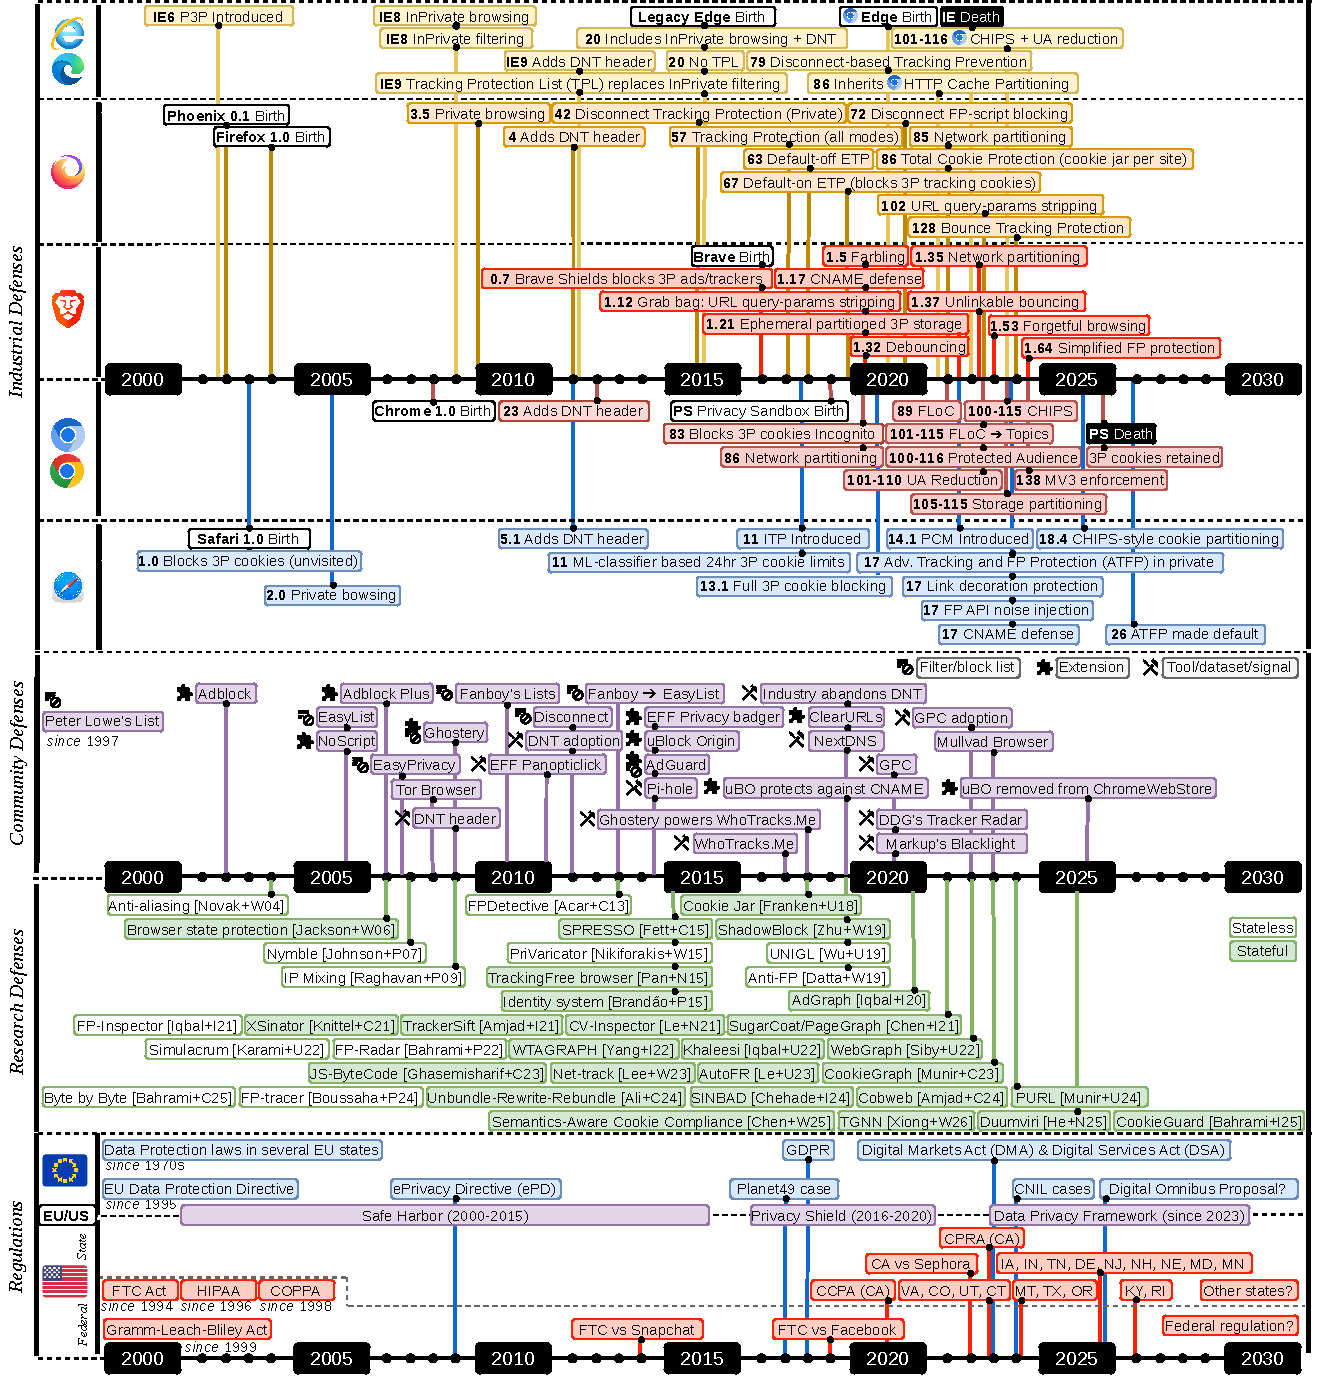
\includegraphics[width=\textwidth]{figures/evolution-tracking-defenses-regulations.pdf}
    \caption{Evolution of \emph{industry-}, \emph{community-}, and \emph{research-based} defenses from 2000--2026 with EU and US \textit{regulations}.}
    \label{fig:evolution-defenses}
\end{figure*}


% \newpage
\begin{table*}[t]
  \scriptsize
\centering
\caption{\textbf{Industrial and community defenses against stateful tracking} across two defense goals: \colorbox{cellred}{detection \& blocking} and \colorbox{cellyellow}{signal reduction \& obfuscation}. Protects against: \iconCookie: Cookie-based tracking, \iconURL: Navigational tracking, \iconFingerprint: Fingerprinting, \iconJS: JavaScript-based tracking, \iconSC: Side-channels. ``(D)'' is by-default, ``(P)'' is private-mode only, and ``(O)'' is opt-in based.}
\label{tab:stateful-tracking-defenses}
\footnotesize
\renewcommand{\arraystretch}{1.1}
\scalebox{0.74}{%
\begin{tabular}{
  m{3.15cm}
  m{3.0cm}
  m{3.0cm}
  m{3.0cm}
  m{3.0cm}
  m{3.0cm}
  m{3.0cm}
}
\toprule
\textbf{Defense Technique}\newline (\textbf{Protects Against}) & \textbf{Brave} & \textbf{Chrome} & \textbf{Edge} & \textbf{Firefox} & \textbf{Safari} & \textbf{Community Defense} \\
\toprule

\cellcolor{cellred} Blocking\newline3P cookies/storage\newline\newline \iconCookie
  & all 3P cookies and storage blocked via Shields (D)
  & 3P cookies and storage blocked in Incognito (P)
  & known tracker 3P cookies blocked (D)
  & known tracker 3P cookies blocked in ETP stnd. (D);\newline all 3P cookies blocked in ETP Strict (D)
  & all 3P cookies and storage blocked (D)
  & Tor blocks 3P cookies and storage\newline uBO, Privacy Badger, AdGuard, Ghostery blocks known tracker cookies via filter lists \\
\midrule

\cellcolor{cellyellow} Partitioning\newline3P cookies/storage\newline\newline \iconCookie\,\iconSC
  & uses Chromium's storage partitioning;\newline ephemeral 3P cookies/storage cleared on tab close (D)
  & opt-in partitioned cookies via \texttt{Partitioned} attribute: CHIPS;\newline storage partitioned by top-level site (D)
  & uses Chromium's CHIPS and its storage partitioning (D)
  & Total Cookie Protection: separate cookie jar per top-level site for all embedded 3P origins;\newline all storage APIs isolated per top-level site (D)
  & \texttt{Partitioned} cookie attribute supported;\newline Access to the 3P storage restricted under ITP;\newline Storage API provides a controlled opt-in (D)
  & ---\\
\midrule

\cellcolor{cellred} Blocking\newline1P tracking cookies/storage\newline\newline \iconCookie
  & Brave Shields blocks 1P-disguised trackers via filter lists (D)
  & NA
  & NA
  & NA
  & ITP purges 1P cookies from classified trackers after inactivity (D)
  & uBO and AdGuard supports targeted deletion of known 1P tracking cookies via filter rules and scriptlets \\
\midrule

\cellcolor{cellyellow} Limiting\newline1P cookie/storage lifetime\newline\newline \iconCookie
  & Caps lifetime of script-set cookies to 7 days;\newline Forgetful Browsing auto-clears 1P storage per-site (O)
  & NA
  & NA
  & NA
  & all script-set 1P cookies/storage expire after 7 days without interaction;\newline Expiry reduced to 24h when link decoration is detected (D)
  & ---\\
\midrule

\cellcolor{cellyellow} HTTP cache partitioning\newline\newline \iconCookie\,\iconSC
  & Inherits Chromium cache partitioning (D)
  & Cache keyed by top-level site (D)
  & Inherits Chromium cache partitioning (D)
  & Network partitioning includes cache isolation per top-level site (D)
  & ITP's isolation addresses cache-based tracking vectors (D)
  & ---\\
\midrule

\cellcolor{cellyellow} Network state partitioning\newline\newline \iconCookie\,\iconURL\,\iconJS\,\iconFingerprint
  & Network state partitioned (D)
  & Included with broader partitioning effort (D)
  & Inherits Chromium network partitioning (D)
  & TLS sessions, DNS cache, HSTS, OCSP, connections all isolated per top-level site (D)
  & Isolation at network-level under ITP's tracking prevention framework (D)
  & ---\\
\midrule

\cellcolor{cellred} URL parameter stripping\newline\newline \iconURL
  & Strips the known tracking query parameters (D)
  & NA
  & NA
  & Query-parameter stripping for known tracking parameters in ETP Strict and Private Browsing (O)
  & ITP detects link decora- tion and reduces script-writable storage lifetime from 7 to 24 hours (D);\newline ATFP's link tracking pro- tection strips params (P)
  & ClearURLs strips utm\_*, gclid, fbclid\newline DuckDuckGo strips by default \\
\midrule

\cellcolor{cellyellow} Referrer policy restrictions\newline\newline \iconURL
  & Strict referrer policy strips cross-origin referrer detail (D)
  & Defaults to strict-origin-when-cross-origin (D)
  & Inherits Chromium referrer policy (D)
  & Defaults to strict-origin-when-cross-origin (D)
  & Defaults to strict-origin-when-cross-origin (D)
  & AdGuard stealth strips referrers;\newline uBO can modify referrer headers via dynamic filtering \\
\midrule

\cellcolor{cellred} Blocking\newline CNAME-cloaked trackers\newline\newline \iconURL\,\iconCookie
  & Blocks CNAME-cloaked trackers (D)
  & NA
  & NA
  & NA;\newline uBO performs CNAME uncloaking through the \texttt{browser.dns} API
  & ITP applies CNAME/IP heuristics for detecting cloaked 3P hosts;\newline ATFP blocks CNAME-cloaked trackers (D)
  & uBO performs CNAME uncloaking (only Firefox);\newline AdGuard does CNAME resolution;\newline Extension-based defenses lack full DNS visibility \\
\midrule

\cellcolor{cellred} Protecting\newline against bounce tracking\newline\newline \iconURL\,\iconCookie
  & Debouncing skips known bounce-tracker redirects;\newline Unlinkable bouncing rou- tes visits through temporary unlinkable storage (D)
  & Heuristics-based deletion of site storage for bounce domains without any recent user interaction (D)
  & NA
  & ETP Strict uses blocklists; deletes storage without recent interaction (D)
  & Behavioral heuristics for deletion of storage for suspected trackers lacking legitimate interaction (D)
  & ---\\
\midrule

\cellcolor{cellred} Blocking known trackers\newline via filter/block lists\newline\newline \iconCookie\,\iconURL\,\iconJS\,\iconFingerprint
  & Shields blocks known 3P ads, trackers, crypto (D)
  & NA
  & Balanced and Strict mode blocks trackers from Disconnect list (D)
  & ETP blocks trackers from Disconnect list (D)
  & ITP and ATFP blocks kn- own and CNAME-cloaked trackers (D)
  & \textit{List}: easylist, easyprivacy, disconnect, Fanboy's lists, Peter Lowe's list, AdGuard lists, DuckDuckGo Tracker Radar;\newline \textit{Extension}: Ghostery, Ad- Guard, Privacy Badger, uBO;\newline \textit{DNS}: Pi-hole, NextDNS \\
\midrule

\cellcolor{cellred} ML-based\newline ad/tracker blocking\newline\newline \iconCookie\,\iconURL\,\iconJS\,\iconFingerprint
  & PageGraph detects trackers via page-level graph analysis (D)
  & NA
  & NA
  & NA
  & ITP uses ML classifier to identify tracking domains from cross-site loading patterns (D)
  & Privacy Badger learns fr- om observed cross-site behavior;\newline Blacklight scans sites for trackers and fingerprinting \\

\bottomrule
\end{tabular}%
}% end scalebox
\end{table*}
\begin{table*}[t]
  \scriptsize
\centering
\caption{\textbf{Industrial and community defenses against stateless tracking} across defense goals: \colorbox{cellred}{detection \& blocking} and \colorbox{cellyellow}{signal reduction \& obfuscation}. Protects against: \iconCookie: Cookie-based tracking, \iconURL: Navigational tracking, \iconFingerprint: Fingerprinting, \iconJS: JavaScript-based tracking, \iconSC: Side-channels. ``(D)'' is by-default, ``(P)'' is private-mode only, and ``(O)'' is opt-in based.}
\label{tab:stateless-tracking-defenses}
\footnotesize
\renewcommand{\arraystretch}{1.1}
\scalebox{0.74}{%
\begin{tabular}{
  m{3.15cm}
  m{3.0cm}
  m{3.0cm}
  m{3.0cm}
  m{3.0cm}
  m{3.0cm}
  m{3.0cm}
}
\toprule
\textbf{Defense Technique}\newline (\textbf{Protects Against}) & \textbf{Brave} & \textbf{Chrome} & \textbf{Edge} & \textbf{Firefox} & \textbf{Safari} & \textbf{Community Defense} \\
\toprule

\cellcolor{cellyellow} Masking or hiding\newline IP address\newline\newline \iconFingerprint
  & Private Window with Tor routes traffic through Tor network (O)
  & IP Protection hides IP via two-hop proxy system (P) (discontinued)
  & NA
  & NA;\newline Mozilla VPN available
  & iCloud's Private Relay routes Safari traffic via two relays to hide IP (O)
  & Tor Browser routes all traffic via onion network \\
\midrule

\cellcolor{cellyellow} Reducing\newline User-Agent string\newline\newline \iconFingerprint
  & Inherits Chromium UA reduction (D)
  & UA reduction and UA Client Hints (D)
  & Inherits Chromium UA reduction and Client Hints (D)
  & Uses the reduced form of Gecko UA string; resist-fingerprinting feature reports generic UA (D)
  & Freezes Safari version in UA string; limits exposed platform detail (D)
  & AdGuard's Stealth Mode can override UA \\
\midrule

\cellcolor{cellred} Blocking\newline fingerprinting scripts\newline\newline \iconJS\,\iconFingerprint
  & PageGraph records page execution for fingerprinting detection;\newline Shields blocks known fingerprinting scripts (D)
  & NA
  & Fingerprinting tracker blo- cking via Disconnect lists (D)
  & Fingerprinting script blo- cking via Disconnect lists (D)
  & ATFP blocks known fingerprinting scripts (P)
  & NoScript blocks JS (D);\newline uBO, AdGuard block fingerprinting domains;\newline Privacy Badger detects fi- ngerprinting-like behavior\\
\midrule

\cellcolor{cellyellow} Normalizing\newline browser API outputs\newline\newline \iconFingerprint
  & NA
  & NA
  & NA
  & resist-fingerprinting standardizes API outputs to uniform values for system specs like hardware and screen metrics (O)
  & ATFP normalizes fonts, plugins, UA (D);\newline ATFP standardizes some outputs such as screen, window, hardware metrics by default in private mode (O)
  & Tor normalizes API outputs for a uniform fingerprint\newline Mullvad Browser applies same hardening for non-Tor use (D) \\
\midrule

\cellcolor{cellyellow} Randomizing\newline browser API outputs\newline\newline \iconFingerprint
  & Farbling does site-specific randomization of API outputs via noise injection so that fingerprint changes per page load (D)
  & NA
  & NA
  & Randomizes API outputs of Canvas, JS floating po- int math operations, and peripheral touch support (D)
  & ATFP injects noise to au-\newline dio, canvas, WebGL by default in private mode (O)
  & ---\\
\midrule

\cellcolor{cellyellow} Reducing precision\newline of browser API outputs\newline\newline \iconFingerprint\,\iconSC
  & Reduces timer's precision (D)
  & Reduces \texttt{performance.now} resolution (D)
  & Inherits Chromium timer precision reductions (D)
  & Reduces event time and \texttt{performance.now}  precision\newline resist-fingerprinting mode applies broader reductions by injecting noise into dynamic hardware hooks like Canvas and timer (D)
  & Reduces timer's precision (D)
  & ---\\
\midrule

\cellcolor{cellred} Removing or declining\newline fingerprintable APIs\newline\newline \iconFingerprint
  & Restricts or disables the fingerprinting-prone APIs where feasible (D)
  & Removed Battery Status API (D)
  & Inherits Chromium API removals (D)
  & Removed Battery Status API; declined Network Information API (D)
  & Declined Network Information API, Web Bluetooth; WebKit policy considers fingerprinting impact for new APIs (D)
  & ---\\
\midrule

\cellcolor{cellred} Blocking JavaScript\newline\newline \iconJS\,\iconFingerprint
  & Brave Shields allows per-site script blocking; aggressive mode blocks all scripts (O)
  & Available via site settings (O)
  & Available via site settings (O)
  & Available via about:config and site permissions (O)
  & Available via site settings (O)
  & NoScript blocks JS by default per-site; highly effective but significant usability burden \\
\midrule

\cellcolor{cellred} Neutralization of\newline mixed scripts\newline\newline \iconJS\,\iconFingerprint\,\iconCookie
  & SugarCoat generates rep-\newline lacement scripts preserv- ing the functionality while neutralizing tracking (D)
  & NA
  & NA
  & NA;\newline uBO scriptlets can override specific functions
  & NA
  & ---\\
\midrule

\cellcolor{cellyellow} Defending against\newline Extension fingerprinting\newline\newline \iconFingerprint
  & Randomizes artifacts detectable by extensions (D)
  & NA
  & NA
  & Extension APIs somewhat isolated but not fully hardened
  & Extensions are run within sandboxed context with limited web-accessible resources (D)
  & ---\\
\midrule

\cellcolor{cellyellow} Side-channel defenses\newline\newline \iconSC
  & Inherits Chromium miti- gations;\newline Shields provides additio-\newline nal isolation (D)
  & Site Isolation COOP/\newline COEP headers;\newline State partitioning (D)
  & Inherits Chromium Site\newline Isolation \& COOP/COEP (D)
  & Site Isolation (Fission);\newline Network partitioning;\newline Reduced timer precision (D)
  & Process-per-tab isolation\newline ITP state partitioning (D)
  & ---\\

\bottomrule
\end{tabular}%
}% end scalebox
\end{table*}


% \newpage
% ── Adjustable parameters ──
\newcommand{\tablescale}{0.8}        % Scale factor for entire table (1.0 = full size)
\newcommand{\rowheight}{1.0}          % Row height multiplier (1.0 = default, lower = tighter)

\newlength{\colBrowser}   \setlength{\colBrowser}{0.7cm}
\newlength{\colDate}      \setlength{\colDate}{2cm}
\newlength{\colVersion}   \setlength{\colVersion}{2.2cm}
\newlength{\colProtects}  \setlength{\colProtects}{2cm}
\newlength{\colDesc}      \setlength{\colDesc}{13.2cm}


\begin{table*}[t]
  \scriptsize
\centering
\caption{\textbf{Evolution of industry-driven tracking defenses across different browsers.} \iconCookie: Cookie-based tracking, \iconURL: Navigational tracking, \iconFingerprint: Fingerprinting, \iconJS: JavaScript-based tracking, \iconSC: Side-channels, \iconPrivacy: Privacy proposals.}
\label{tab:defenses-industrial}
\footnotesize
\renewcommand{\arraystretch}{\rowheight}
\scalebox{\tablescale}{%
\begin{tabular}{
  >{\centering\arraybackslash}m{\colBrowser}
  >{\centering\arraybackslash}m{\colDate}
  >{\centering\arraybackslash}m{\colVersion}
  >{\centering\arraybackslash}m{\colProtects}
  m{\colDesc}
}
\toprule
\textbf{Browser} & \textbf{Release Date} & \textbf{Browser Version} & \textbf{Protects Against} & \textbf{Description of the Introduced Tracking Defenses} \\
\toprule

% ─────────────────────────────────────────────
%  INTERNET EXPLORER  (4 rows)
% ─────────────────────────────────────────────
% multirow vertical centering: adjust the value in brackets [Xpt]
% positive = shift up, negative = shift down
\multirow{4}{*}[0pt]{\iconIE}
  & Aug 2001 & 6  & \iconCookie                                & P3P support; 3P cookies restricted by default unless an acceptable P3P compact policy is present \\
  & Mar 2009 & 8  & \iconCookie\,\iconSC       & Introduced InPrivate Browsing and InPrivate Filtering (blocks 3P content loaded across $>$10 sites) \\
  % ; also clears some Flash supercookies \\
  & Mar 2011 & 9  & \iconCookie\,\iconURL\,\iconFingerprint  & Tracking Protection Lists (TPL) replaces InPrivate Filtering; Do Not Track (DNT) support added \\
  & Jun 2022 & 11 &       ---       & Last IE~11 desktop app retired and disabled, redirecting to Microsoft Edge \\
\midrule

% ─────────────────────────────────────────────
%  EDGE  (7 rows)
% ─────────────────────────────────────────────
\multirow{7}{*}[-5pt]{\iconEdge}
  & Jul 2015    & 20      & --- & Edge launches with Windows~10, InPrivate browsing, and DNT; drops IE's TPL \\
  & Jan 2020    & 79      & \iconCookie\,\iconURL\,\iconFingerprint & Chromium Edge with Disconnect-based blocking; blocks cryptomining+fingerprinting trackers \\
  & Oct 2020    & 86      & \iconSC                                  & Inherits Chromium HTTP cache partitioning \\
  & 2022--2023  & 101--116 & \iconFingerprint\, \iconPrivacy                           & Inherits Chromium User-Agent reduction (reduced UA string; UA Client Hints) \\
  & May 2023    & 114     & \iconCookie\,\iconSC\, \iconPrivacy                     & Inherits Chromium CHIPS (partitioned 3P cookies) \\
  & Aug 2023    & 115     & \iconSC                                  & Inherits Chromium Storage Partitioning \\
  & Jun 2024    & 139     & ---                                & Inherits Chromium Manifest~V3 enforcement; MV2 ad/tracker blockers phased out \\
\midrule

% ─────────────────────────────────────────────
%  FIREFOX  (14 rows)
% ─────────────────────────────────────────────
\multirow{14}{*}[-15pt]{\iconFirefox}
  & Sep 2002 & 0.1       & \iconCookie                                 & Launch of Phoenix~0.1 with basic cookie management \\
  & Nov 2004 & 1         & \iconCookie                                 & Launch of Firefox~1.0: cookie manager with exceptions; option to block 3P cookies \\
  & Jun 2009 & 3.5       & ---                                  & Private Browsing mode introduced \\
  & Mar 2011 & 4         & ---                             & Do Not Track (DNT) header adopted; first browser to implement DNT \\
  & Nov 2015 & 42        & \iconCookie\,\iconURL\,\iconFingerprint          & Tracking Protection blocks known trackers in Private Browsing using Disconnect list \\
  & Nov 2017 & 57        & \iconCookie\,\iconURL\,\iconFingerprint                   & Tracking Protection available outside Private Browsing (optional) \\
  & Oct 2018 & 63        & \iconCookie\,\iconJS          & Enhanced Tracking Protection (ETP) introduced (off by default) \\
  & Jun 2019 & 67        & \iconCookie\,\iconJS                                 & ETP turned on by default for new installs (Standard mode) \\
  & Jan 2020 & 72        & \iconFingerprint\,\iconJS                   & Fingerprinting-script blocking enabled by default via Disconnect's fingerprinting list \\
  & Jul 2020 & 79        & \iconURL                                    & Basic redirect (bounce) tracking protection introduced \\
  & Jan 2021 & 85        & \iconCookie\,\iconSC                     & Supercookie protection via network partitioning (caches/connections isolated per top-level site) \\
  & Feb 2021 & 86        & \iconCookie                     & Total Cookie Protection introduced (separate cookie jar per website under ETP Strict) \\
  & Jun 2022 & 102       & \iconURL                                    & URL query-parameter stripping for known tracking parameters (ETP Strict and Private Browsing) \\
  & Aug 2024     & 128       & \iconURL                                    & Bounce Tracking Protection introduced to ETP Strict \\
\midrule

% ─────────────────────────────────────────────
%  SAFARI  (10 rows)
% ─────────────────────────────────────────────
\multirow{10}{*}[-15pt]{\iconSafari}
  & Jun 2003 & 1    & \iconCookie                                          & Launch of Safari~1.0: blocks 3P cookies from unvisited sites by default \\
  & Apr 2005 & 2    & ---                                           & Private Browsing mode introduced; first browser to offer it \\
  & Jul 2011     & 5.1  & ---                                      & DNT header support added \\
  & Sep 2017 & 11   & \iconCookie                         & ITP~1.0: ML identifies tracking cookies; 24h 3P cookie window; purges 30d+ unused cookies \\
  & Sep 2019 & 13   & \iconURL\,\iconJS\,\iconSC                        & ITP~2.3: 7-day cap on all script-writable storage to counter storage and link-decoration tracking \\
  & Mar 2020 & 13.1 & \iconCookie                                          & Complete 3P cookie blocking enabled by default; first mainstream browser to block all 3P cookies \\
  & Apr 2021 & 14.1 & \iconPrivacy                        & Private Click Measurement (PCM) enabled by default for privacy-preserving ad click attribution \\
  & Sep 2023 & 17   & \iconCookie\,\iconURL\,\iconFingerprint\ & Advanced Tracking and Fingerprinting Protection (ATFP) in Private Browsing: Link Tracking Protection, API noise injection, blocks known/CNAME-cloaked trackers \\
  & Mar 2025 & 18.4 & \iconCookie\,\iconSC                              & Support for the CHIPS-styled partitioned cookie attribute introduced \\
  & Sep 2025 & 26   & \iconFingerprint                                     & Advanced Fingerprinting Protection extended to default (non-Private) browsing \\
\midrule

% ─────────────────────────────────────────────
%  CHROME  (14 rows)
% ─────────────────────────────────────────────
\multirow{14}{*}[-15pt]{\iconChrome}
  & Dec 2008 & 1              & ---                    & Launch of Chrome~1.0 stable: Incognito mode \\
  & Nov 2012 & 23             & ---               & DNT header support added \\
  & Aug 2019 & ---            & \iconPrivacy                  & Privacy Sandbox initiative announced \\
  & May 2020 & 83             & \iconCookie\       & 3P cookies blocked by default in Incognito mode; new cookie controls \\
  & Oct 2020 & 86             & \iconSC                    & HTTP cache partitioning (cache keyed by top-level site) \\
  & Apr 2021 & 89             & \iconPrivacy & FLoC origin trial begins (interest cohorts as a 3P cookie alternative) \\
  & Jan 2022 & 101--115 (OT)  
  & \iconPrivacy                  & FLoC abandoned; Topics API proposed as replacement \\
  & Apr 2022 & 100--116 (OT)  
  & \iconPrivacy & FLEDGE in-browser ad-auction origin trial begins \\
  & Jun 2022 & 101--110 (OT)  
  & \iconFingerprint\,\iconPrivacy              & UA Reduction introduced: browser minor version reduced to 0.0.0 in the UA string \\
  & May 2023 & 100--115 (OT)  
  & \iconCookie\,\iconSC,\iconPrivacy & CHIPS (Cookies Having Independent Partitioned State) introduced \\
  & Aug 2023 & 105--115 (OT)  
  & \iconSC                    & Storage Partitioning (localStorage, IndexedDB, CacheStorage partitioned by top-level site) \\
  & Apr 2025 & ---            & \iconCookie\,\iconPrivacy     & Google drops planned 3P cookie prompt; cookies remain; deprecation effort ended \\
  & Sep 2025 & 138            & ---                  & Manifest~V3 enforcement; MV2 ad/tracker blockers phased out \\
  & Oct 2025 & ---            & \iconPrivacy                  & Privacy Sandbox APIs (Topics, Protected Audience, Attribution Reporting, etc.) retired \\
\midrule

% ─────────────────────────────────────────────
%  BRAVE  (11 rows)
% ─────────────────────────────────────────────
\multirow{11}{*}[-10pt]{\iconBrave}
  & Jan 2016 & 0.7  & \iconCookie\,\iconURL\,\iconFingerprint\,\iconSC & Developer preview: blocks 3P ads/trackers and 3P storage by default; HTTPS Everywhere \\
  & Nov 2019 & 1    & \iconCookie\,\iconURL\,\iconFingerprint\,\iconSC           & Launch of Brave~1.0: Shields blocks 3P ads/trackers, cross-site cookies, and fingerprinting by default \\
  & Mar 2020 & 1.5  & \iconFingerprint                                        & Fingerprint randomization (farbling) introduced \\
  & Jul 2020 & 1.12 & \iconURL                                                & URL query-parameter stripping, stricter referrer policy, Reporting API limits \\
  & Jul 2020 & 1.17 & \iconCookie\,\iconURL\,\iconFingerprint                                & Defense against CNAME-cloaked trackers \\
  & Feb 2021 & 1.21 & \iconCookie\,\iconSC                                 & Ephemeral 3P site storage (partitioned and cleared when site closes) \\
  & Oct 2021 & 1.32 & \iconURL                                                & Debouncing introduced; skips known bounce-tracker redirects \\
  & Dec 2021 & 1.35 & \iconCookie\,\iconSC                                 & Partitioning of network state \\
  & Mar 2022 & 1.37 & \iconURL                                                & Unlinkable Bouncing: routes suspected-site visits through temporary, unlinkable storage \\
  & May 2023 & 1.53 & \iconCookie\,\iconSC                                 & Forgetful Browsing: auto-clear first-party storage per-site \\
  & Jan 2024 & 1.64 & \iconFingerprint                                        & Simplified fingerprinting protections \\

\bottomrule
\end{tabular}%
}% end scalebox
\end{table*}
% ── Column widths (community-defense table) ──
\newlength{\colCYear}    \setlength{\colCYear}{0.5cm}
\newlength{\colCName}    \setlength{\colCName}{3.8cm}
\newlength{\colCType}    \setlength{\colCType}{0.6cm}
\newlength{\colCDesc}    \setlength{\colCDesc}{15.5cm}


\begin{table*}[t]
  \scriptsize
\centering
\caption{\textbf{Timeline of community-driven tracking defenses.} \iconBlocklist: Filter/block list, \iconExtension: Browser extension, \iconTool: represents tools, standards, dataset, or browser.}
\label{tab:defenses-community}
\footnotesize
\renewcommand{\arraystretch}{\rowheight}
\scalebox{\tablescale}{%
\begin{tabular}{
  >{\centering\arraybackslash}m{\colCYear}
  m{\colCName}
  >{\centering\arraybackslash}m{\colCType}
  m{\colCDesc}
}
\toprule
\textbf{Year} & \textbf{Community Defense} & \textbf{Type} & \textbf{Description} \\
\toprule

1997 & Peter Lowe's list (pgl.yoyo.org) & \iconBlocklist & Initially created for personal local DNS use, this crowdsourced adblock list is widely consumed by hosts files, Pi-hole, AdGuard, uBO \\
2002 & Adblock & \iconExtension & Ad blocking extension created for Firefox; later replaced by its successors \\
2005 & EasyList & \iconBlocklist & Created as a maintainable ad-blocking subscription for the Adblock extension; has become the de-facto core ad filter list \\
2005 & NoScript & \iconExtension & Blocks JavaScript content by default per-site, cutting JS-based tracking and fingerprinting \\
2006 & Adblock Plus (Eyeo) & \iconExtension & Adblock extension re-written as Adblock Plus with subscribable filter lists (e.g.\ EasyList) \\
2006 & EasyPrivacy & \iconBlocklist & Companion list to EasyList targeting trackers, analytics, tracking pixels/beacons, and web bugs (not just ads) \\
2008 & Tor Browser (Tor Project) & \iconTool & Reference anti-fingerprinting and onion-routing browser; provides first-party isolation and uniform fingerprint (one-fingerprint-for-all) \\
2009 & Ghostery & \iconExtension & Detects and (optionally) blocks 3P trackers; also exposes who is tracking on each page \\
2009 & Do Not Track (DNT) & \iconTool & Proposed by researchers as a browser header to opt out of cross-site tracking \\
2010 & Fanboy's Annoyance List & \iconBlocklist & List targeting cookie-consent notices, social-media widgets, and in-page annoyances (basis for EasyList Cookie List) \\
2010 & EFF Panopticlick & \iconTool & EFF tool demonstrating browser fingerprint uniqueness and tracker exposure \\
2011 & Disconnect & \iconBlocklist & List blocks 3P trackers; its open tracker list got later on adopted by Firefox, Safari, and Edge \\
2011 & Do Not Track (DNT) & \iconTool & Implemented by Firefox, IE, Safari, Opera, then Chrome; W3C Tracking Protection WG chartered to standardize it \\
2013 & Fanboy $\rightarrow$ EasyList & \iconBlocklist & Fanboy's List merged into EasyList, consolidating the dominant English ad-filter lists \\
2014 & Privacy Badger (EFF) & \iconExtension & Heuristic tracker blocker that learns about trackers from observed cross-site behavior rather than a static list \\
2014 & uBlock Origin & \iconExtension & uBlock released for Chrome/Opera \\
2014 & AdGuard & \iconBlocklist\,\iconExtension & Extension blocks ad/tracker domains based on various lists; Stealth Mode strips referrers, 3P cookies, and reduces fingerprinting surface \\
2014 & Pi-hole & \iconTool & Open-source network-wide DNS sinkhole (Raspberry Pi); blocks ad/tracker domains for an entire network via DNS \\
2017 & WhoTracks.me & \iconTool & Open dataset and reporting of trackers' prevalence and behavior across the web \\
2018 & Ghostery powers WhoTracks.Me & \iconTool & Ghostery goes open source; powers the WhoTracks.me tracker dataset \\
2019 & Do Not Track (DNT) & \iconTool & W3C Tracking Protection Working Group closed without DNT adoption; DNT effectively abandoned by industry \\
2019 & ClearURLs & \iconExtension & Strips known tracking parameters (e.g.\ utm\_*, gclid, fbclid) from URLs before requests and on copy \\
2019 & NextDNS & \iconTool & Cloud DNS resolver with configurable ad/tracker blocklists, applied across devices/browsers \\
2019 & uBO protects against CNAME & \iconExtension & uBO (Firefox) adds CNAME-uncloaking to defeat first-party-disguised (CNAME-cloaked) trackers; advanced dynamic filtering/scriptlets \\
2020 & Global Privacy Control (GPC) & \iconTool & EFF-led universal opt-out signal; legally enforceable under CCPA/CPRA; adopted by DuckDuckGo, Brave, Abine, Firefox \\
2020 & DuckDuckGo Tracker Radar & \iconTool & Open, auto-generated tracker dataset (domains $\rightarrow$ owners $\rightarrow$ behaviors); powers DDG protections, Vivaldi, and Blacklight \\
2020 & Blacklight & \iconTool & Markup's web tool that scans any site and reports trackers, cookies, session recorders, pixels, and fingerprinting \\
2022 & GPC Adoption & \iconTool & California Sephora settlement establishes that ignoring GPC violates CCPA, driving site adoption \\
2023 & Mullvad Browser & \iconTool & Tor Project + Mullvad: Tor Browser's anti-fingerprinting hardening for everyday (non-Tor-network) use \\
2025 & uBO removed from Chrome & \iconExtension & uBO removed from the Chrome Web Store as Chrome disables MV2 extensions by July 2025; remains full-featured on Firefox/Brave \\

\bottomrule
\end{tabular}%
}% end scalebox
\end{table*}

% \newpage
\begin{table*}[!ht]
  \small
  \centering
  \caption{Taxonomy of policies along with their distribution across the literature (\# = paper count).}
  \label{tab:regulations-paper-distribution}
\begin{subtable}[t]{0.29\linewidth}
\centering
  \begin{tabular}{>{\centering\arraybackslash}p{4cm} >{\centering\arraybackslash}p{0.1cm}}
    \toprule
    \multicolumn{1}{c}{\textbf{EU Regulation}} & \multicolumn{1}{l}{\textbf{\#}} \\
    \midrule
    GDPR & 27 \\
    ePrivacy Directive (ePD) & 9 \\
    Digital Services Act (DSA) & 3 \\
    Digital Markets Act (DMA) & 1 \\
    \bottomrule
  \end{tabular}
  \caption{EU Regulations}
\end{subtable}
\begin{subtable}[t]{0.29\linewidth}
\centering
  \begin{tabular}{>{\centering\arraybackslash}p{4cm} >{\centering\arraybackslash}p{0.1cm}}
    \toprule
    \multicolumn{1}{c}{\textbf{US Regulation}} & \multicolumn{1}{l}{\textbf{\#}} \\
    \midrule
    CCPA (California) & 11 \\
    CPRA (California) & 3 \\
    Other states & 2 \\
    FTC Act or COPPA (Federal) & 2\\
    \bottomrule
  \end{tabular}
  \caption{US Regulations}
\end{subtable}
\begin{subtable}[t]{0.4\linewidth}
\centering
  \begin{tabular}{>{\centering\arraybackslash}p{6cm} >{\centering\arraybackslash}p{0.1cm}}
    \toprule
    \multicolumn{1}{c}{\textbf{Standard}} & \multicolumn{1}{l}{\textbf{\#}} \\
    \midrule
    GPC & 5 \\
    P3P & 3\\
    DNT & 3 \\
    IAB TCF or CCPA Compliance Framework & 3 \\
    \bottomrule
  \end{tabular}
  \caption{Opt-Out Signals and Industry Frameworks}
\end{subtable}
\end{table*}
\begin{table*}[!ht]
    \small
    \centering
    \caption{Taxonomy of policy aspects (along with its distribution across literature) mapped onto rights and context applicability.}
    \label{tab:regulations-aspects}
    % \setlength{\tabcolsep}{2pt}
    % \renewcommand{\arraystretch}{.7}
    \begin{tabular}{cccccccccc}
    \toprule
    && \multicolumn{6}{c}{\textbf{Right to}} \\
    \textbf{Policy Aspect} & \rot{\textbf{\# Paper count}} &\rot{\textbf{Access}} &\rot{\textbf{Portability}} &\rot{\textbf{Correct}} &\rot{\textbf{Delete}} &\rot{\textbf{Opt-out}} &\rot{\textbf{Consent}} & \textbf{GDPR/ePD Context} & \textbf{CCPA/CPRA Context}\\
    \midrule

    User Consent & 18 & \pie{0} & \pie{0} & \pie{0} & \pie{0} & \pie{0} & \pie{360} & \checkmark\ Opt-in design & \xmark\ Opt-out design\\

    Notice & 8 & \pie{360} & \pie{0} & \pie{0} & \pie{0} & \pie{0} & \pie{360} & \checkmark\ Prelude for consent & \checkmark\ Disclosure requirements \\

    Sharing \& Consent Propagation & 7 & \pie{0} & \pie{0} & \pie{0} & \pie{360} & \pie{360} & \pie{360} & \checkmark\ Processor obligations & \xmark\ Third-party notices\\

    Opt-out Sale & 6 & \pie{0} & \pie{0} & \pie{0} & \pie{360} & \pie{360} & \pie{0} & \xmark\ Opt-in design & \checkmark\ Opt-out design\\

    Data Access Request & 5 & \pie{360} & \pie{360} & \pie{360} & \pie{360} & \pie{0} & \pie{0} & \checkmark\ Controller must provide info. & \checkmark\ Requests to know \\

    Data Minimization & 4 & \pie{360} & \pie{360} & \pie{360} & \pie{360} & \pie{360} & \pie{360} & \checkmark\ Processing principle & \checkmark\ CPRA amendment \\

    Legitimate Interest Exemption & 5 & \pie{0} & \pie{0} & \pie{0} & \pie{0} & \pie{360} & \pie{360} & \checkmark\ Specific purposes only& \xmark\ No equivalent\\

    Data Storage (persistence) & 3 & \pie{360} & \pie{360} & \pie{360} & \pie{360} & \pie{0} & \pie{0} & \checkmark\ Storage limitations & \checkmark\ Retention schedules\\

    Privacy by Design & 1 & \pie{0} & \pie{360} & \pie{360} & \pie{0} & \pie{0} & \pie{360} & \checkmark\ By design and by default & \checkmark\ CPRA amendment\\

     \bottomrule
    \end{tabular}
\end{table*}

